\documentclass[conference]{IEEEtran}
\usepackage[utf8]{inputenc}
\usepackage{cite}
\usepackage{amsmath,amssymb,amsfonts}
\usepackage{graphicx}
\usepackage{textcomp}
\usepackage{xcolor}
\usepackage{float}
\usepackage{geometry}
\usepackage{afterpage}
\usepackage{pdfpages}
\usepackage{verbatim}
\usepackage{listings}

\begin{document}

% ==========================================================
% HALAMAN COVER (BERDASARKAN COVER.DOCX)
% ==========================================================
\begin{titlepage}
\onecolumn
\centering
\thispagestyle{empty}

\vspace*{0.5cm}

{\fontsize{16pt}{22pt}\selectfont\bfseries LAPORAN PROGRESS\par}
\vspace{0.4cm}
{\fontsize{14pt}{18pt}\selectfont\bfseries Mata Kuliah Workshop Pemrograman Framework\par}
\vspace{0.3cm}
{\fontsize{14pt}{18pt}\selectfont\bfseries Dokumen PRD\par}

\vfill


\includegraphics[width=7.5cm]{pens_logo.png}\par

\vfill

{\fontsize{12pt}{16pt}\selectfont\bfseries Dosen Pengampu:\par}
\vspace{0.2cm}
{\fontsize{12pt}{16pt}\selectfont Amma Liesvarastranta Haz, S.Tr.T., M.T.\par}

\vspace{0.8cm}

{\fontsize{12pt}{16pt}\selectfont\bfseries Disusun Oleh:\par}
\vspace{0.25cm}
{\fontsize{12pt}{16pt}\selectfont 1. Ahmad Falihul Hikam (3125521007)\par}
\vspace{0.15cm}
{\fontsize{12pt}{16pt}\selectfont 2. Arvin Dzaky Nugraha (3125521027)\par}

\vfill

{\fontsize{13pt}{18pt}\selectfont\bfseries PROGRAM STUDI D3 TEKNIK INFORMATIKA\par}
\vspace{0.15cm}
{\fontsize{13pt}{18pt}\selectfont\bfseries DEPARTEMEN TEKNIK INFORMATIKA DAN KOMPUTER\par}
\vspace{0.15cm}
{\fontsize{13pt}{18pt}\selectfont\bfseries POLITEKNIK ELEKTRONIKA NEGERI SURABAYA\par}
\vspace{0.2cm}
{\fontsize{13pt}{18pt}\selectfont\bfseries 2026\par}

\vspace*{0.5cm}
\end{titlepage}
\clearpage
\twocolumn

\title{SIGAP: Sistem Informasi Pengaduan Perundungan dan Kekerasan Pelajar Berbasis Platform Digital dan Kecerdasan Buatan}

\author{
\IEEEauthorblockN{Ahmad Falihul Hikam}
\IEEEauthorblockA{\textit{D3 Teknik Informatika PSDKU Lamongan} \\
\textit{Politeknik Elektronika Negeri Surabaya}}
\and
\IEEEauthorblockN{Arvin Dzaky Nugraha}
\IEEEauthorblockA{\textit{D3 Teknik Informatika PSDKU Lamongan} \\
\textit{Politeknik Elektronika Negeri Surabaya}}
}

\maketitle

\begin{abstract}
Perundungan (\textit{bullying}) dan \textit{cyberbullying} di lingkungan pendidikan merupakan isu serius yang berdampak negatif terhadap kesejahteraan psikologis dan perkembangan sosial siswa. Penanganan kasus perundungan sering kali terkendala oleh tiadanya saluran pelaporan yang aman, terstruktur, dan akuntabel, serta kompleksitas verifikasi laporan pada pihak sekolah. Penelitian ini mengajukan SIGAP (Sistem Informasi Pengaduan Perundungan dan Kekerasan Pelajar), sebuah platform digital terpadu yang memfasilitasi pelaporan pengaduan siswa baik secara anonim maupun teridentifikasi, dilengkapi dengan sistem penjejak tiket (\textit{ticket tracking}). SIGAP mengintegrasikan pemrosesan bahasa alami (\textit{Natural Language Processing}/NLP) berbasis \textit{embedding} teks Bahasa Indonesia untuk memberikan rekomendasi pengkategorian laporan secara otomatis guna membantu administrator dalam mengambil keputusan secara efisien. Sistem ini juga dilengkapi dengan mekanisme verifikasi, pengelolaan alur status laporan, dan jejak audit (\textit{audit trail}) untuk menjamin transparansi serta akuntabilitas. Hasil perancangan menunjukkan bahwa SIGAP mampu menyediakan sarana pendukung pelaporan dan pengelolaan perundungan di lingkungan sekolah secara lebih terstruktur, sistematis, dan terukur.
\end{abstract}

\begin{IEEEkeywords}
Perundungan Pelajar, SIGAP, Sistem Pengaduan, Kecerdasan Buatan, Natural Language Processing.
\end{IEEEkeywords}

\section{BAB I: LATAR BELAKANG}

Perkembangan teknologi informasi dan komunikasi telah memberikan kemudahan bagi pelajar dalam berkomunikasi dan berinteraksi, tetapi di sisi lain juga menghadirkan bentuk perundungan baru melalui media digital atau \textit{cyberbullying}. Perundungan tidak hanya terjadi secara langsung di lingkungan sekolah, tetapi dapat berkembang melalui media sosial dan platform digital. Zhang et al. menjelaskan bahwa selama dua dekade terakhir terdapat berbagai definisi dan metode pengukuran \textit{cyberbullying} pada anak dan remaja, yang menunjukkan bahwa fenomena tersebut menjadi perhatian dalam lingkungan digital \cite{zhang2022}. Penelitian Amanatin dan Sekarningrum juga menunjukkan adanya berbagai bentuk dan penyebab \textit{cyberbullying} pada remaja di wilayah perkotaan Indonesia, termasuk Jakarta, Bandung, dan Surabaya \cite{amanatin2024}.

Lingkungan sekolah memiliki peran penting dalam upaya pencegahan dan penanganan perundungan. Maftuh et al. menunjukkan adanya keterkaitan antara iklim sekolah dengan perilaku \textit{cyberbullying} pada siswa sekolah menengah, sehingga kondisi lingkungan sekolah menjadi salah satu aspek yang perlu diperhatikan dalam menangani permasalahan tersebut \cite{maftuh2024}. Selain itu, penelitian Eleanora dan Al Adawiah pada siswa SMK menunjukkan pentingnya upaya preventif dalam menghadapi \textit{cyberbullying} di lingkungan pendidikan \cite{eleanora2021}. Hal ini menunjukkan bahwa sekolah membutuhkan mekanisme yang dapat membantu siswa menyampaikan informasi mengenai perundungan serta membantu pihak sekolah dalam mengelola laporan secara lebih terstruktur.

Perundungan juga dapat memberikan dampak yang serius terhadap siswa. Li et al. melalui meta-analisis menunjukkan adanya hubungan antara \textit{traditional bullying} dan \textit{cyberbullying} dengan berbagai permasalahan kesehatan mental pada anak dan remaja \cite{li2024}. Sementara itu, Evangelio et al. melalui \textit{systematic review} mengenai \textit{cyberbullying} pada siswa sekolah dasar dan menengah menekankan pentingnya upaya pencegahan dan intervensi terhadap permasalahan tersebut \cite{evangelio2022}. Kajian Kasturiratna et al. juga menunjukkan bahwa \textit{cyberbullying} memiliki berbagai faktor risiko, faktor protektif, konsekuensi, serta membutuhkan bentuk intervensi yang sesuai \cite{kasturiratna2025}. Oleh karena itu, diperlukan mekanisme pelaporan yang dapat membantu siswa menyampaikan pengaduan dengan lebih mudah dan membantu pihak sekolah dalam melakukan proses penanganan secara sistematis.

Berdasarkan permasalahan tersebut, diperlukan sebuah sistem informasi yang dapat menjadi media pelaporan sekaligus membantu proses pengelolaan pengaduan perundungan dan kekerasan pelajar. SIGAP (Sistem Informasi Pengaduan Perundungan dan Kekerasan Pelajar) dirancang untuk menyediakan mekanisme pelaporan secara anonim maupun non-anonim, pemberian tiket pengaduan, pemantauan status laporan, serta pengelolaan laporan oleh administrator. Sistem ini juga dirancang dengan pemanfaatan teknologi kecerdasan buatan untuk membantu memberikan rekomendasi kategori berdasarkan isi laporan dan mengelompokkan laporan yang memiliki karakteristik serupa. Dengan adanya SIGAP, proses pelaporan diharapkan menjadi lebih terstruktur, terdokumentasi, dan mudah dipantau, sementara keputusan akhir mengenai verifikasi dan tindak lanjut tetap dilakukan oleh pihak yang berwenang.

\begin{thebibliography}{00}

\bibitem{zhang2022}
W. Zhang, S. Huang, L. Lam, R. Evans, and C. Zhu, ``Cyberbullying definitions and measurements in children and adolescents: Summarizing 20 years of global efforts,'' \textit{Frontiers in Public Health}, vol. 10, 2022, Art. no. 1000504, doi: 10.3389/fpubh.2022.1000504.

\bibitem{amanatin2024}
E. L. Amanatin and B. Sekarningrum, ``Causes and Forms of Cyberbullying among Teenagers in Indonesian Urban Areas: Cases of Jakarta, Bandung and Surabaya,'' \textit{JISPO Jurnal Ilmu Sosial dan Ilmu Politik}, vol. 13, no. 2, pp. 233--254, 2024, doi: 10.15575/jispo.v13i2.27792.

\bibitem{maftuh2024}
B. Maftuh, A. Dahliyana, E. Malihah, and R. Sartika, ``Does school climate matter in cyberbullying behaviour among high school student? A mediation and moderation analysis,'' \textit{Jurnal Cakrawala Pendidikan}, vol. 43, no. 1, pp. 28--43, 2024, doi: 10.21831/cp.v43i1.65213.

\bibitem{li2024}
C. Li, P. Wang, M. Martin-Moratinos, M. Bella-Fernández, and H. Blasco-Fontecilla, ``Traditional bullying and cyberbullying in the digital age and its associated mental health problems in children and adolescents: A meta-analysis,'' \textit{European Child \& Adolescent Psychiatry}, vol. 33, pp. 2895--2909, 2024, doi: 10.1007/s00787-022-02128-x.

\bibitem{evangelio2022}
C. Evangelio, P. Rodríguez-González, J. Fernández-Río, and S. Gonzalez-Villora, ``Cyberbullying in elementary and middle school students: A systematic review,'' \textit{Computers \& Education}, vol. 176, 2022, Art. no. 104356, doi: 10.1016/j.compedu.2021.104356.

\bibitem{kasturiratna2025}
K. T. A. S. Kasturiratna, A. Hartanto, C. H. Y. Chen, E. M. W. Tong, et al., ``Umbrella review of meta-analyses on the risk factors, protective factors, consequences and interventions of cyberbullying victimization,'' \textit{Nature Human Behaviour}, vol. 9, pp. 101--132, 2025, doi: 10.1038/s41562-024-02011-6.

\bibitem{eleanora2021}
F. N. Eleanora and R. A. Al Adawiah, ``Perundungan dunia maya (Cyberbullying) dan upaya preventif di kalangan siswa SMK Bangun Persada Bekasi,'' \textit{Jurnal Abdi Masyarakat Indonesia}, vol. 1, no. 2, pp. 203--208, 2021, doi: 10.54082/jamsi.67.

\end{thebibliography}

% ===== Mulai bagian non-IEEE: satu kolom, tanpa nomor halaman =====
\clearpage
\onecolumn
\pagestyle{empty}

\begin{center}
	{\Large\bfseries BAB II}\par
	\vspace{0.3cm}
	{\Large\bfseries SOURCE CODE}\par
\end{center}

\lstinputlisting[
	language={[LaTeX]TeX},
	basicstyle=\ttfamily\footnotesize,
	breaklines=true,
	breakatwhitespace=false,
	columns=fullflexible,
	keepspaces=true,
	literate={é}{{\'e}}1 {ó}{{\'o}}1 {á}{{\'a}}1 {í}{{\'i}}1,
	frame=single,
	framerule=0.3pt,
	rulecolor=\color{black!35},
	xleftmargin=1cm,
	xrightmargin=1cm,
	framexleftmargin=4pt,
	framexrightmargin=4pt
]{SIGAP-source.tex}

\clearpage
\begin{center}
	{\Large\bfseries BAB III}\par
	\vspace{0.3cm}
	{\Large\bfseries ARSITEKTUR SISTEM}\par
\end{center}

SIGAP menggunakan arsitektur aplikasi web yang terdiri atas frontend,
backend core, lapisan AI/ML, dan data layer. Siswa dan admin mengakses
aplikasi melalui antarmuka React. Permintaan dikirim melalui REST API ke
backend FastAPI untuk autentikasi, pengelolaan laporan, dashboard, dan
komunikasi dengan basis data.

Lapisan AI memproses deskripsi laporan menggunakan embedding Bahasa
Indonesia, cosine similarity, dan HDBSCAN. AI menghasilkan rekomendasi
kategori serta kelompok laporan yang memiliki pola serupa. Keputusan
akhir tetap dilakukan oleh admin yang berwenang.

\begin{figure}[H]
	\centering
	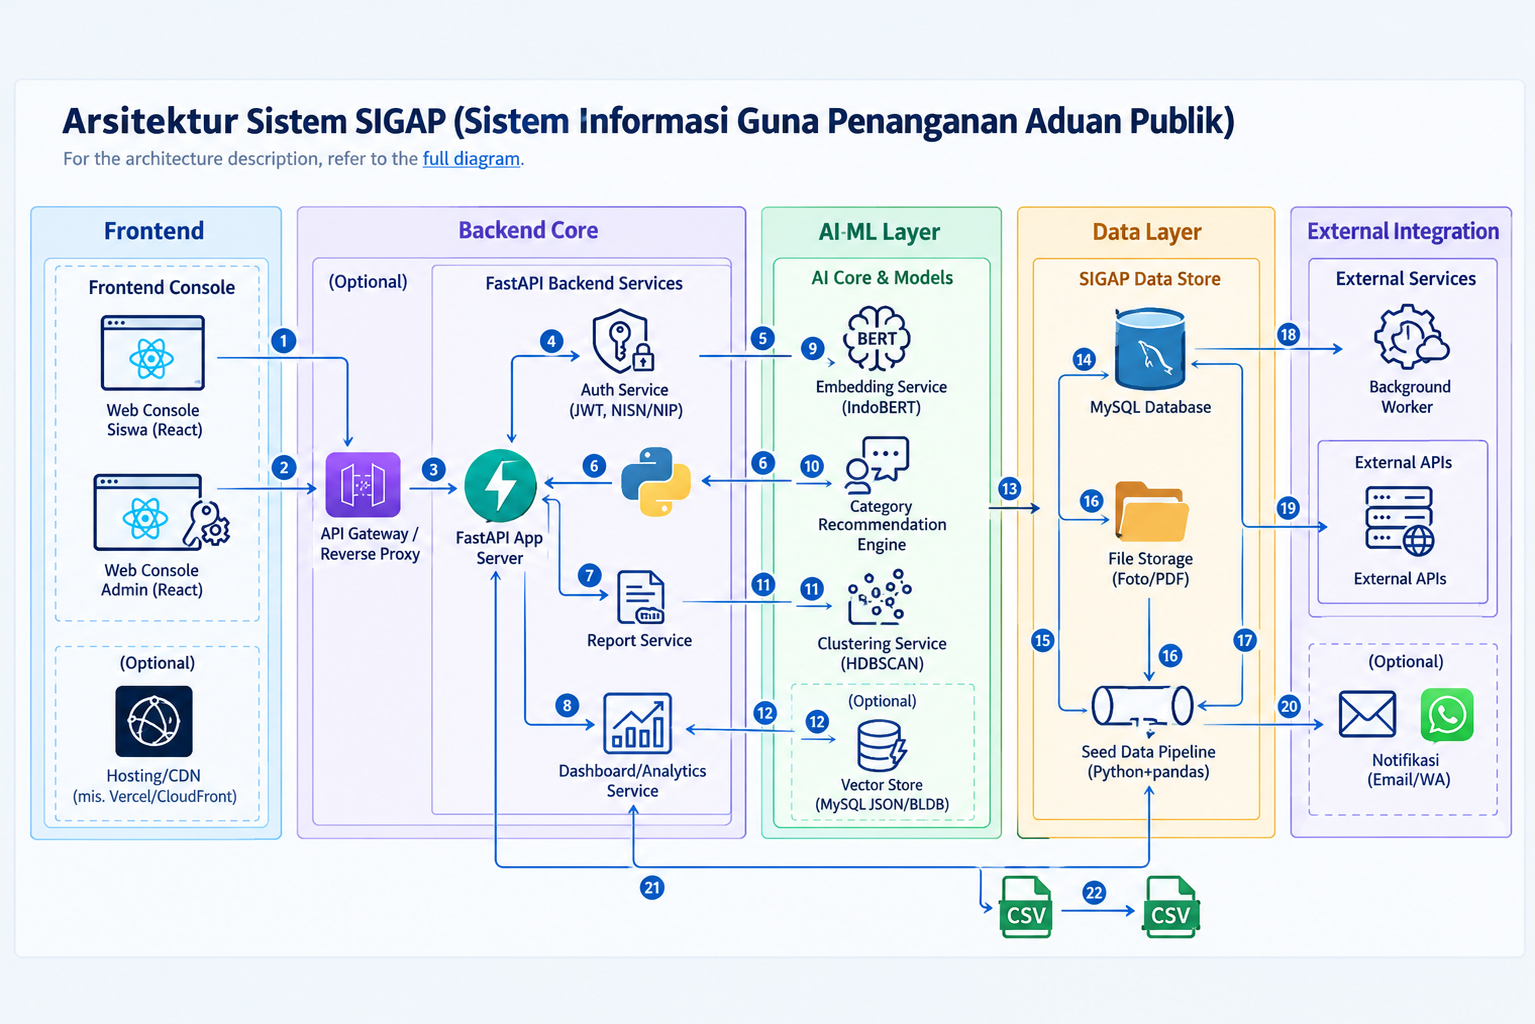
\includegraphics[width=\linewidth,height=0.72\textheight,keepaspectratio]{Arsitektur Sistem SIGAP/ArsitekturSistem_SIGAP.png}
	\caption{Arsitektur Sistem SIGAP}
	\label{fig:arsitektur-sigap}
\end{figure}

Komponen utama sistem meliputi React Student Console, React Admin
Console, FastAPI, JWT Authentication, Report Service, MySQL, file
storage, dan pemrosesan AI. Data laporan menjadi sumber utama sistem,
sedangkan audit trail menyimpan admin, waktu, dan tindakan yang dilakukan.

\subsection*{3.1 Alur Data}

Siswa mengisi laporan, mengunggah bukti bila tersedia, lalu sistem
menyimpan laporan dan menghasilkan ticket ID. Backend meneruskan deskripsi
ke layanan AI untuk memperoleh rekomendasi kategori. Admin meninjau isi
laporan, memvalidasi kategori, dan memperbarui status sesuai state machine.

\subsection*{3.2 Keamanan Sistem}

Keamanan sistem menggunakan HTTPS, JWT, role-based authorization,
validasi tipe dan ukuran file, serta pembatasan akses data anonim. Ticket
tracking tidak menampilkan informasi identitas sensitif kepada pengguna.

\clearpage
\begin{center}
	{\Large\bfseries BAB IV}\par
	\vspace{0.3cm}
	{\Large\bfseries DESAIN SISTEM}\par
\end{center}

Desain SIGAP dibuat dengan karakter aman, bersih, formal, dan mudah
dipahami. Antarmuka siswa menggunakan pendekatan mobile-first, sedangkan
dashboard admin menggunakan pendekatan desktop-first. Warna utama yang
digunakan adalah baby blue \texttt{\#A7D8F0}, putih, serta warna netral untuk
teks, border, dan status.

\begin{figure}[H]
	\centering
	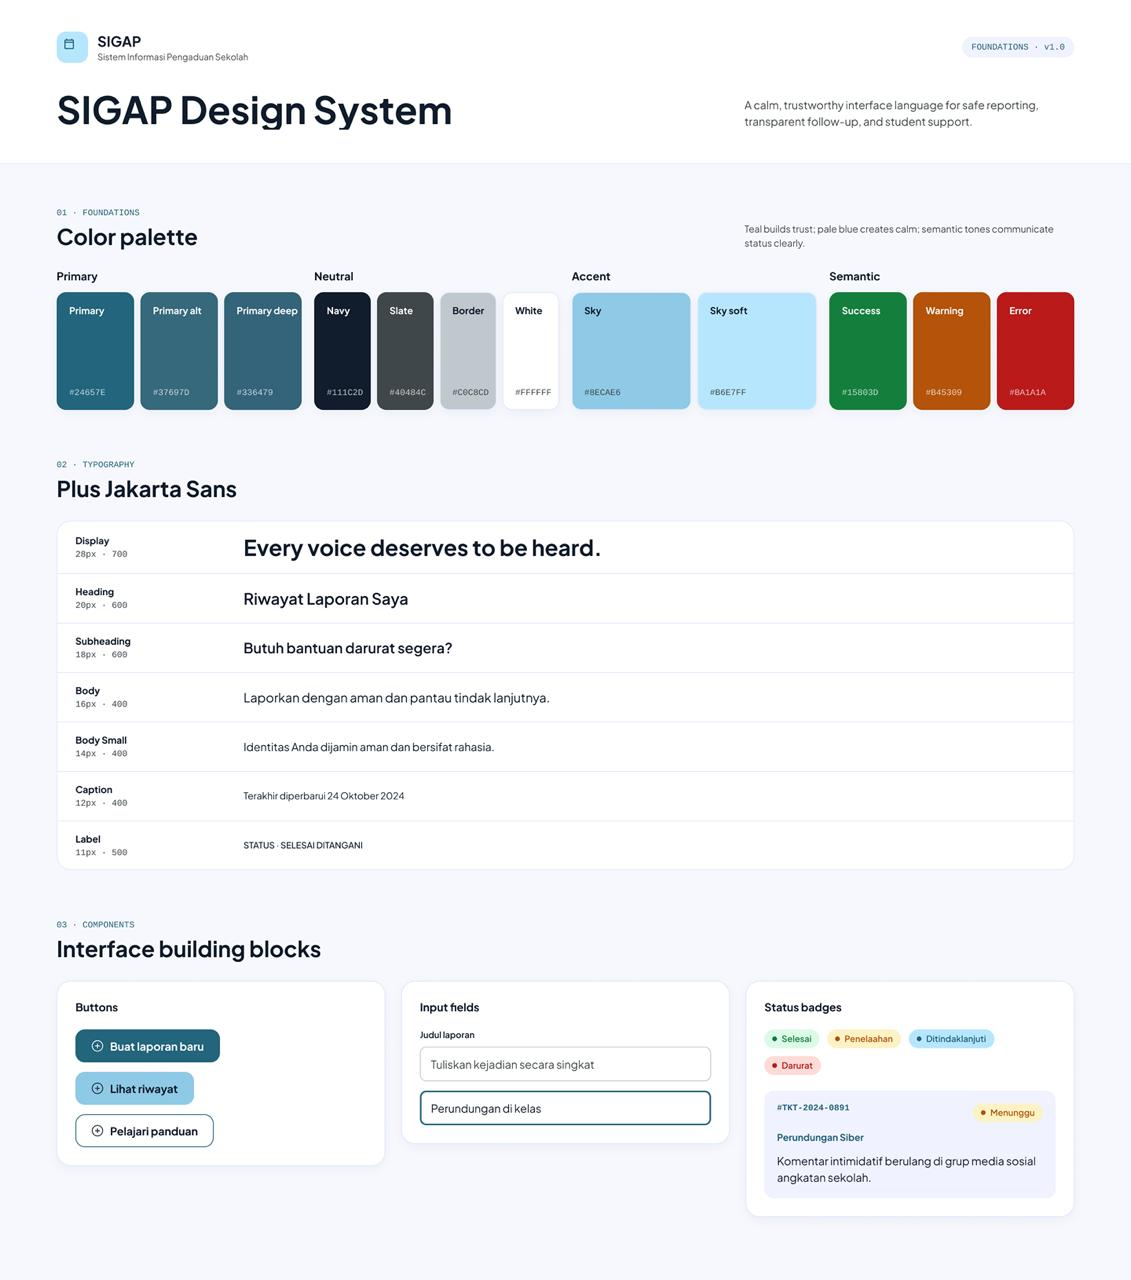
\includegraphics[width=\linewidth,height=0.72\textheight,keepaspectratio]{Desain Sistem/DesainSistem_SIGAP.png}
	\caption{Desain Sistem SIGAP}
	\label{fig:desain-sigap}
\end{figure}

Desain sistem mencakup alur pengaduan siswa, dashboard admin, validasi
rekomendasi AI, pengelolaan status, cluster laporan, dan audit trail.
Navigasi siswa terdiri atas Beranda, Buat Laporan, Riwayat, dan Profil.
Navigasi admin terdiri atas Dashboard, Daftar Laporan, Validasi AI, Audit
Trail, dan Pengaturan.

\subsection*{4.1 Alur Pengaduan}

Formulir pengaduan dibagi menjadi kategori, deskripsi, mode pelaporan,
dan bukti. Siswa dapat memilih pelaporan anonim atau menggunakan nama.
Setelah laporan terkirim, sistem menampilkan kode tiket untuk pelacakan.

\subsection*{4.2 Status dan AI}

Status ditampilkan dengan timeline Menunggu, Diverifikasi,
Ditindaklanjuti, dan Selesai. Rekomendasi AI diberi label khusus dan
confidence. Jika confidence rendah, sistem menampilkan status Perlu
Peninjauan Manual.

\clearpage
\begin{center}
	{\Large\bfseries BAB V}\par
	\vspace{0.3cm}
	{\Large\bfseries MOCKUP UI}\par
\end{center}

Bab ini menampilkan seluruh mockup antarmuka SIGAP yang tersedia pada
folder \texttt{Frontend}. Mockup mencakup alur pengguna siswa dan pengelolaan
laporan oleh admin.

% --- 2 gambar per baris ---
\noindent
\begin{minipage}[t]{0.48\linewidth}
	\begin{figure}[H]
		\centering
		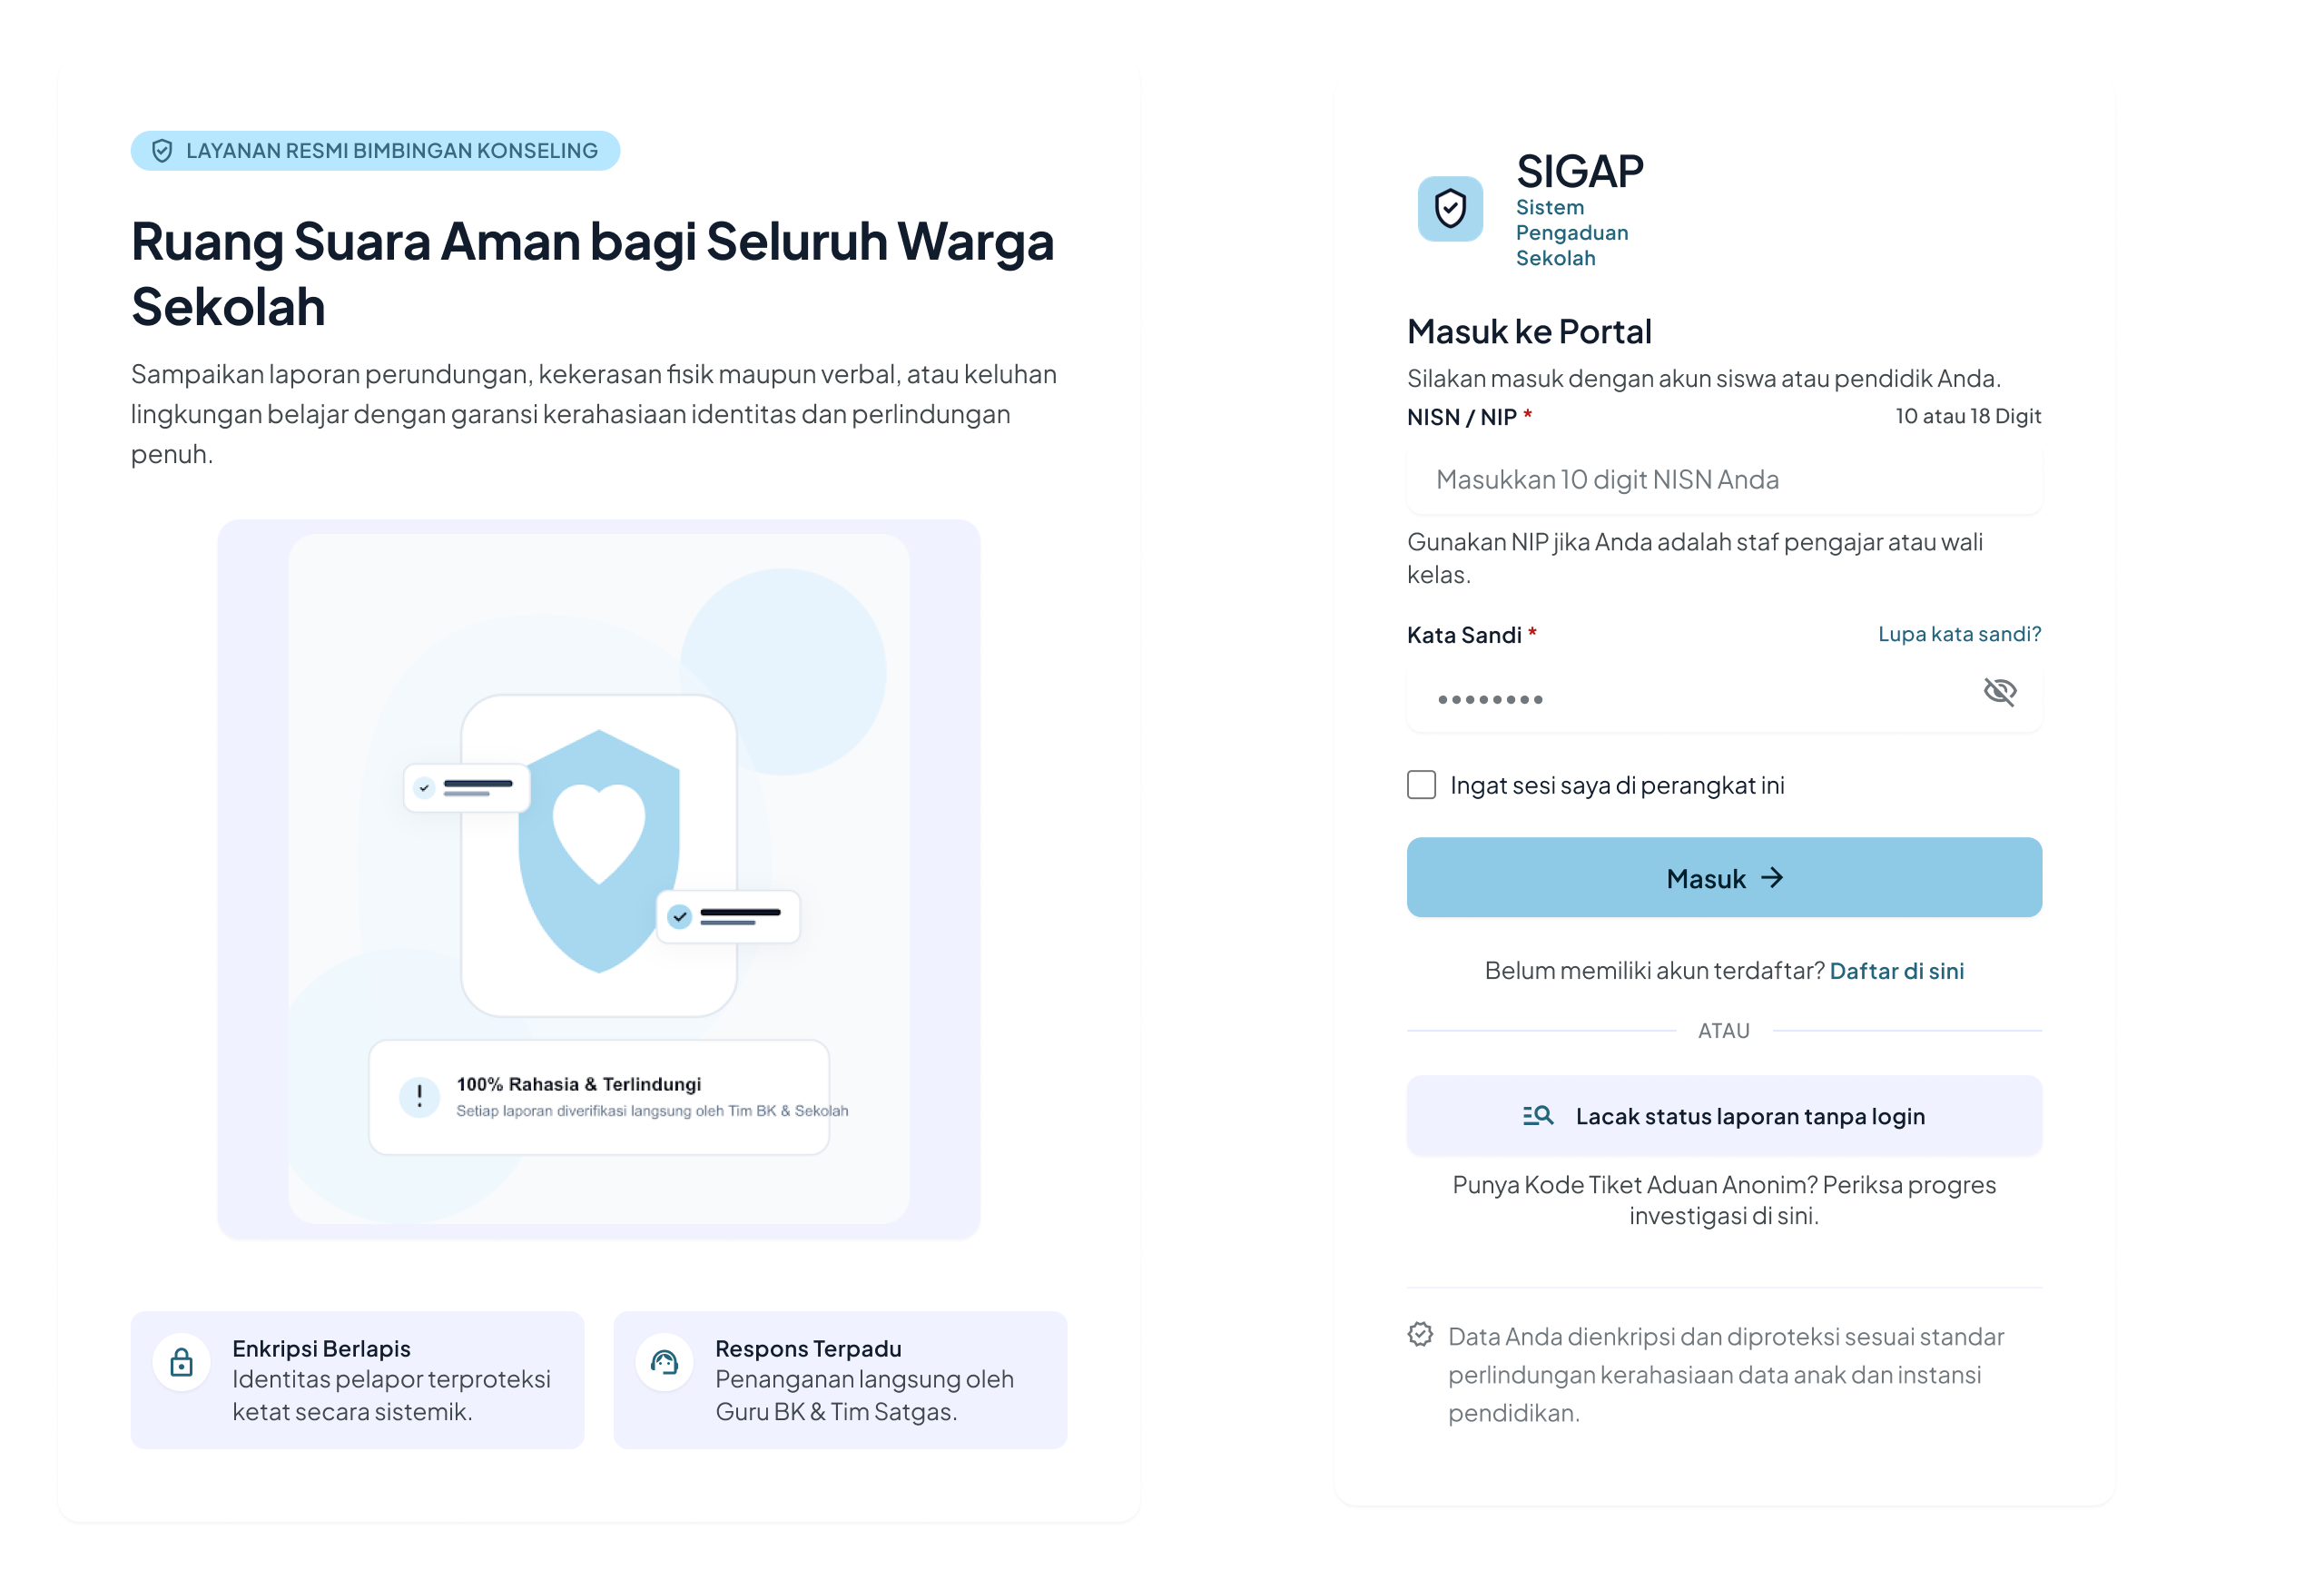
\includegraphics[width=\linewidth,height=0.42\textheight,keepaspectratio]{Frontend/OnBoardingUser_SIGAP.png}
		\caption{Onboarding pengguna siswa}
	\end{figure}
\end{minipage}
\hfill
\begin{minipage}[t]{0.48\linewidth}
	\begin{figure}[H]
		\centering
		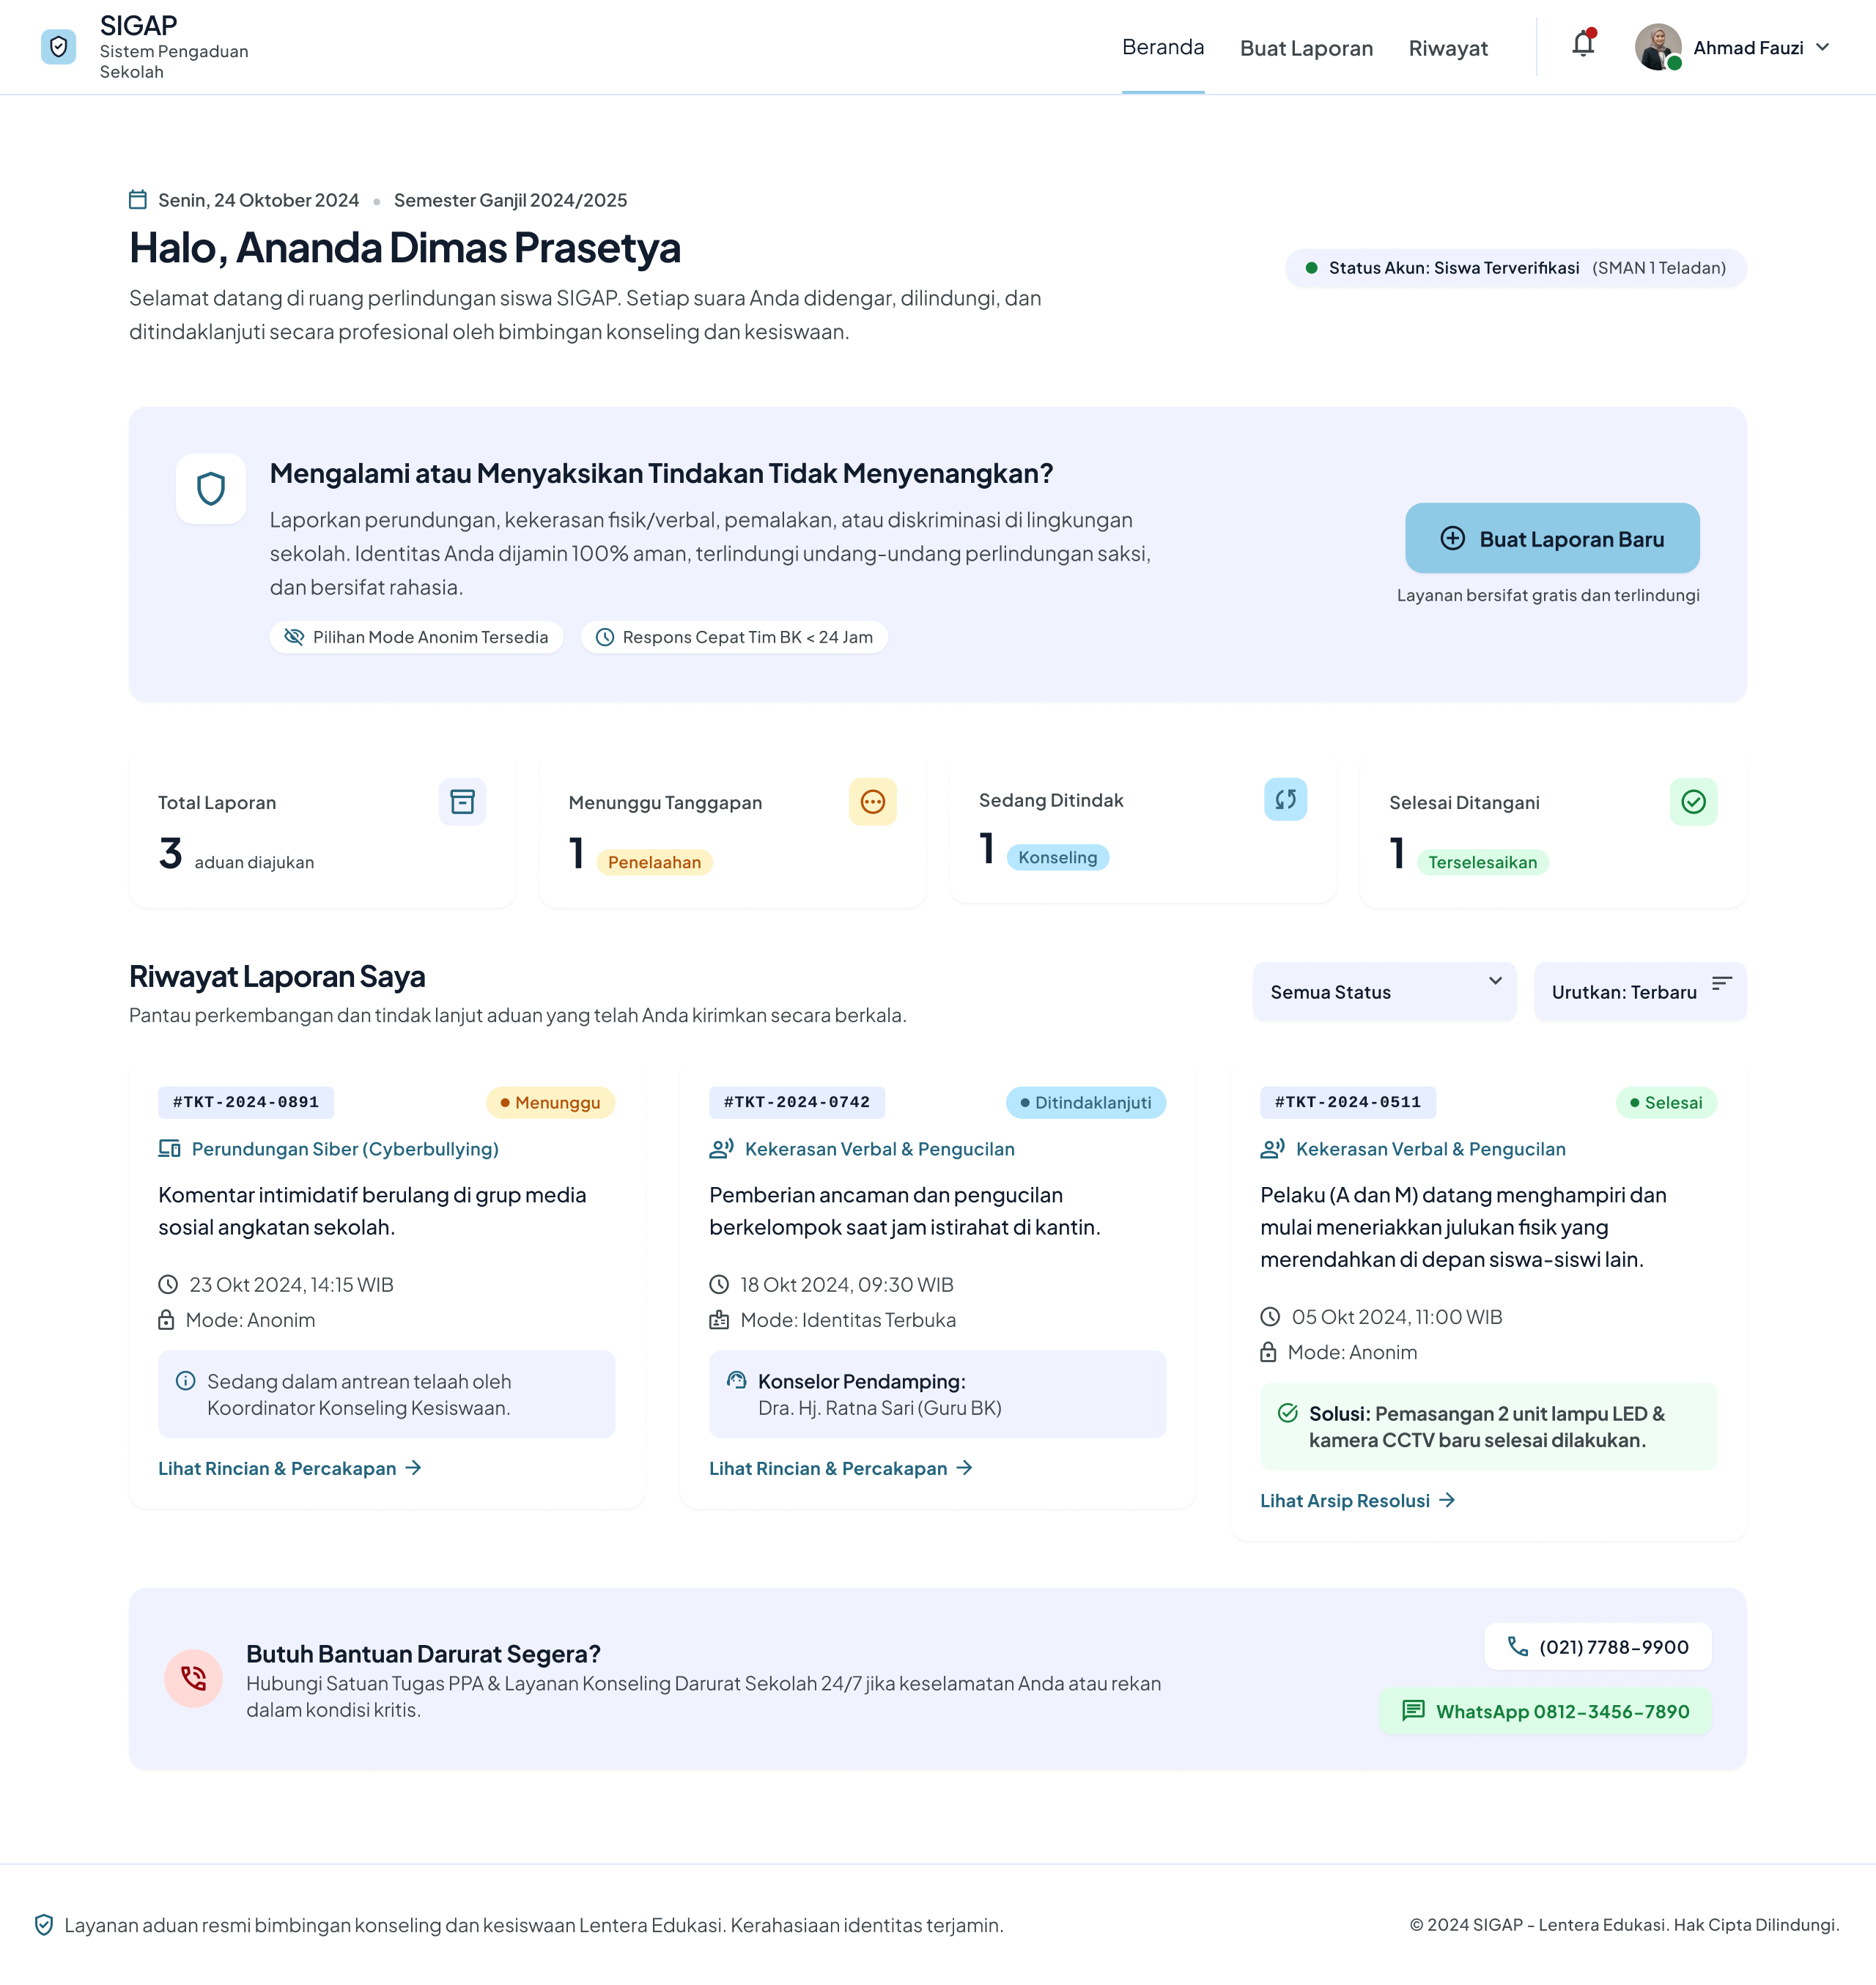
\includegraphics[width=\linewidth,height=0.42\textheight,keepaspectratio]{Frontend/DashboardUser_SIGAP.png}
		\caption{Dashboard pengguna siswa}
	\end{figure}
\end{minipage}

\noindent
\begin{minipage}[t]{0.48\linewidth}
	\begin{figure}[H]
		\centering
		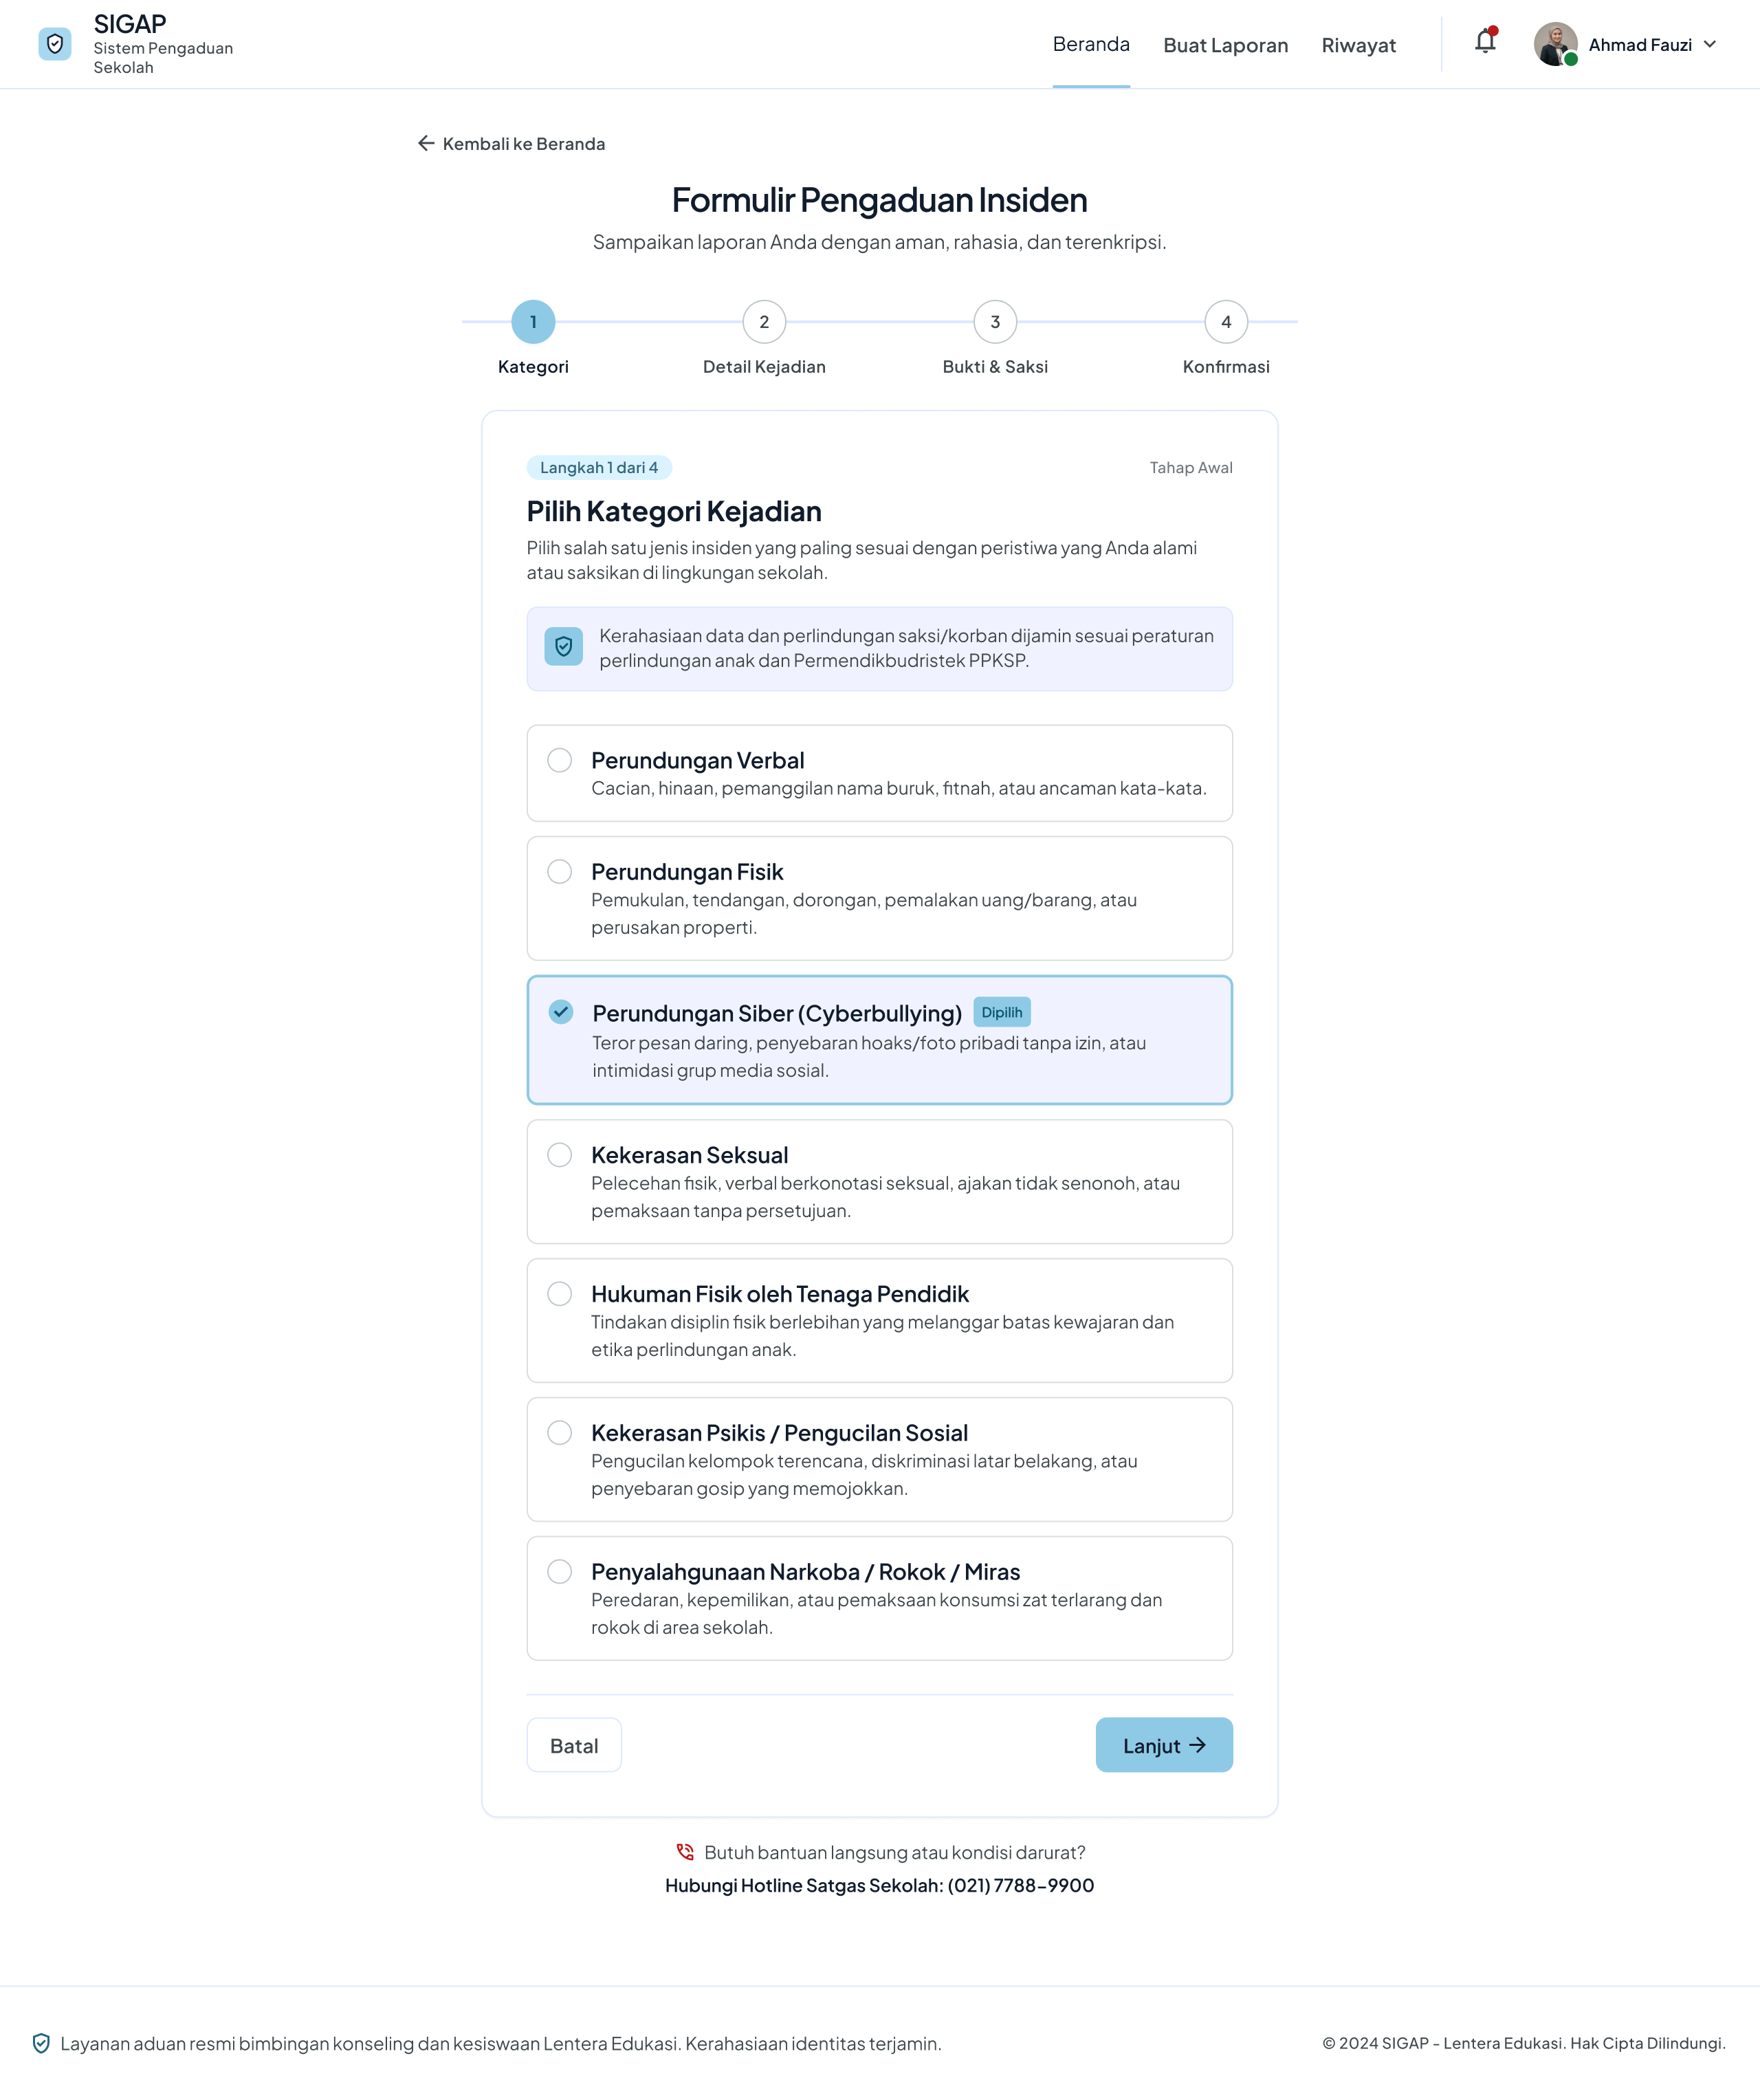
\includegraphics[width=\linewidth,height=0.42\textheight,keepaspectratio]{Frontend/FormulirPengaduanUser_SIGAP.png}
		\caption{Formulir pengaduan pengguna siswa}
	\end{figure}
\end{minipage}
\hfill
\begin{minipage}[t]{0.48\linewidth}
	\begin{figure}[H]
		\centering
		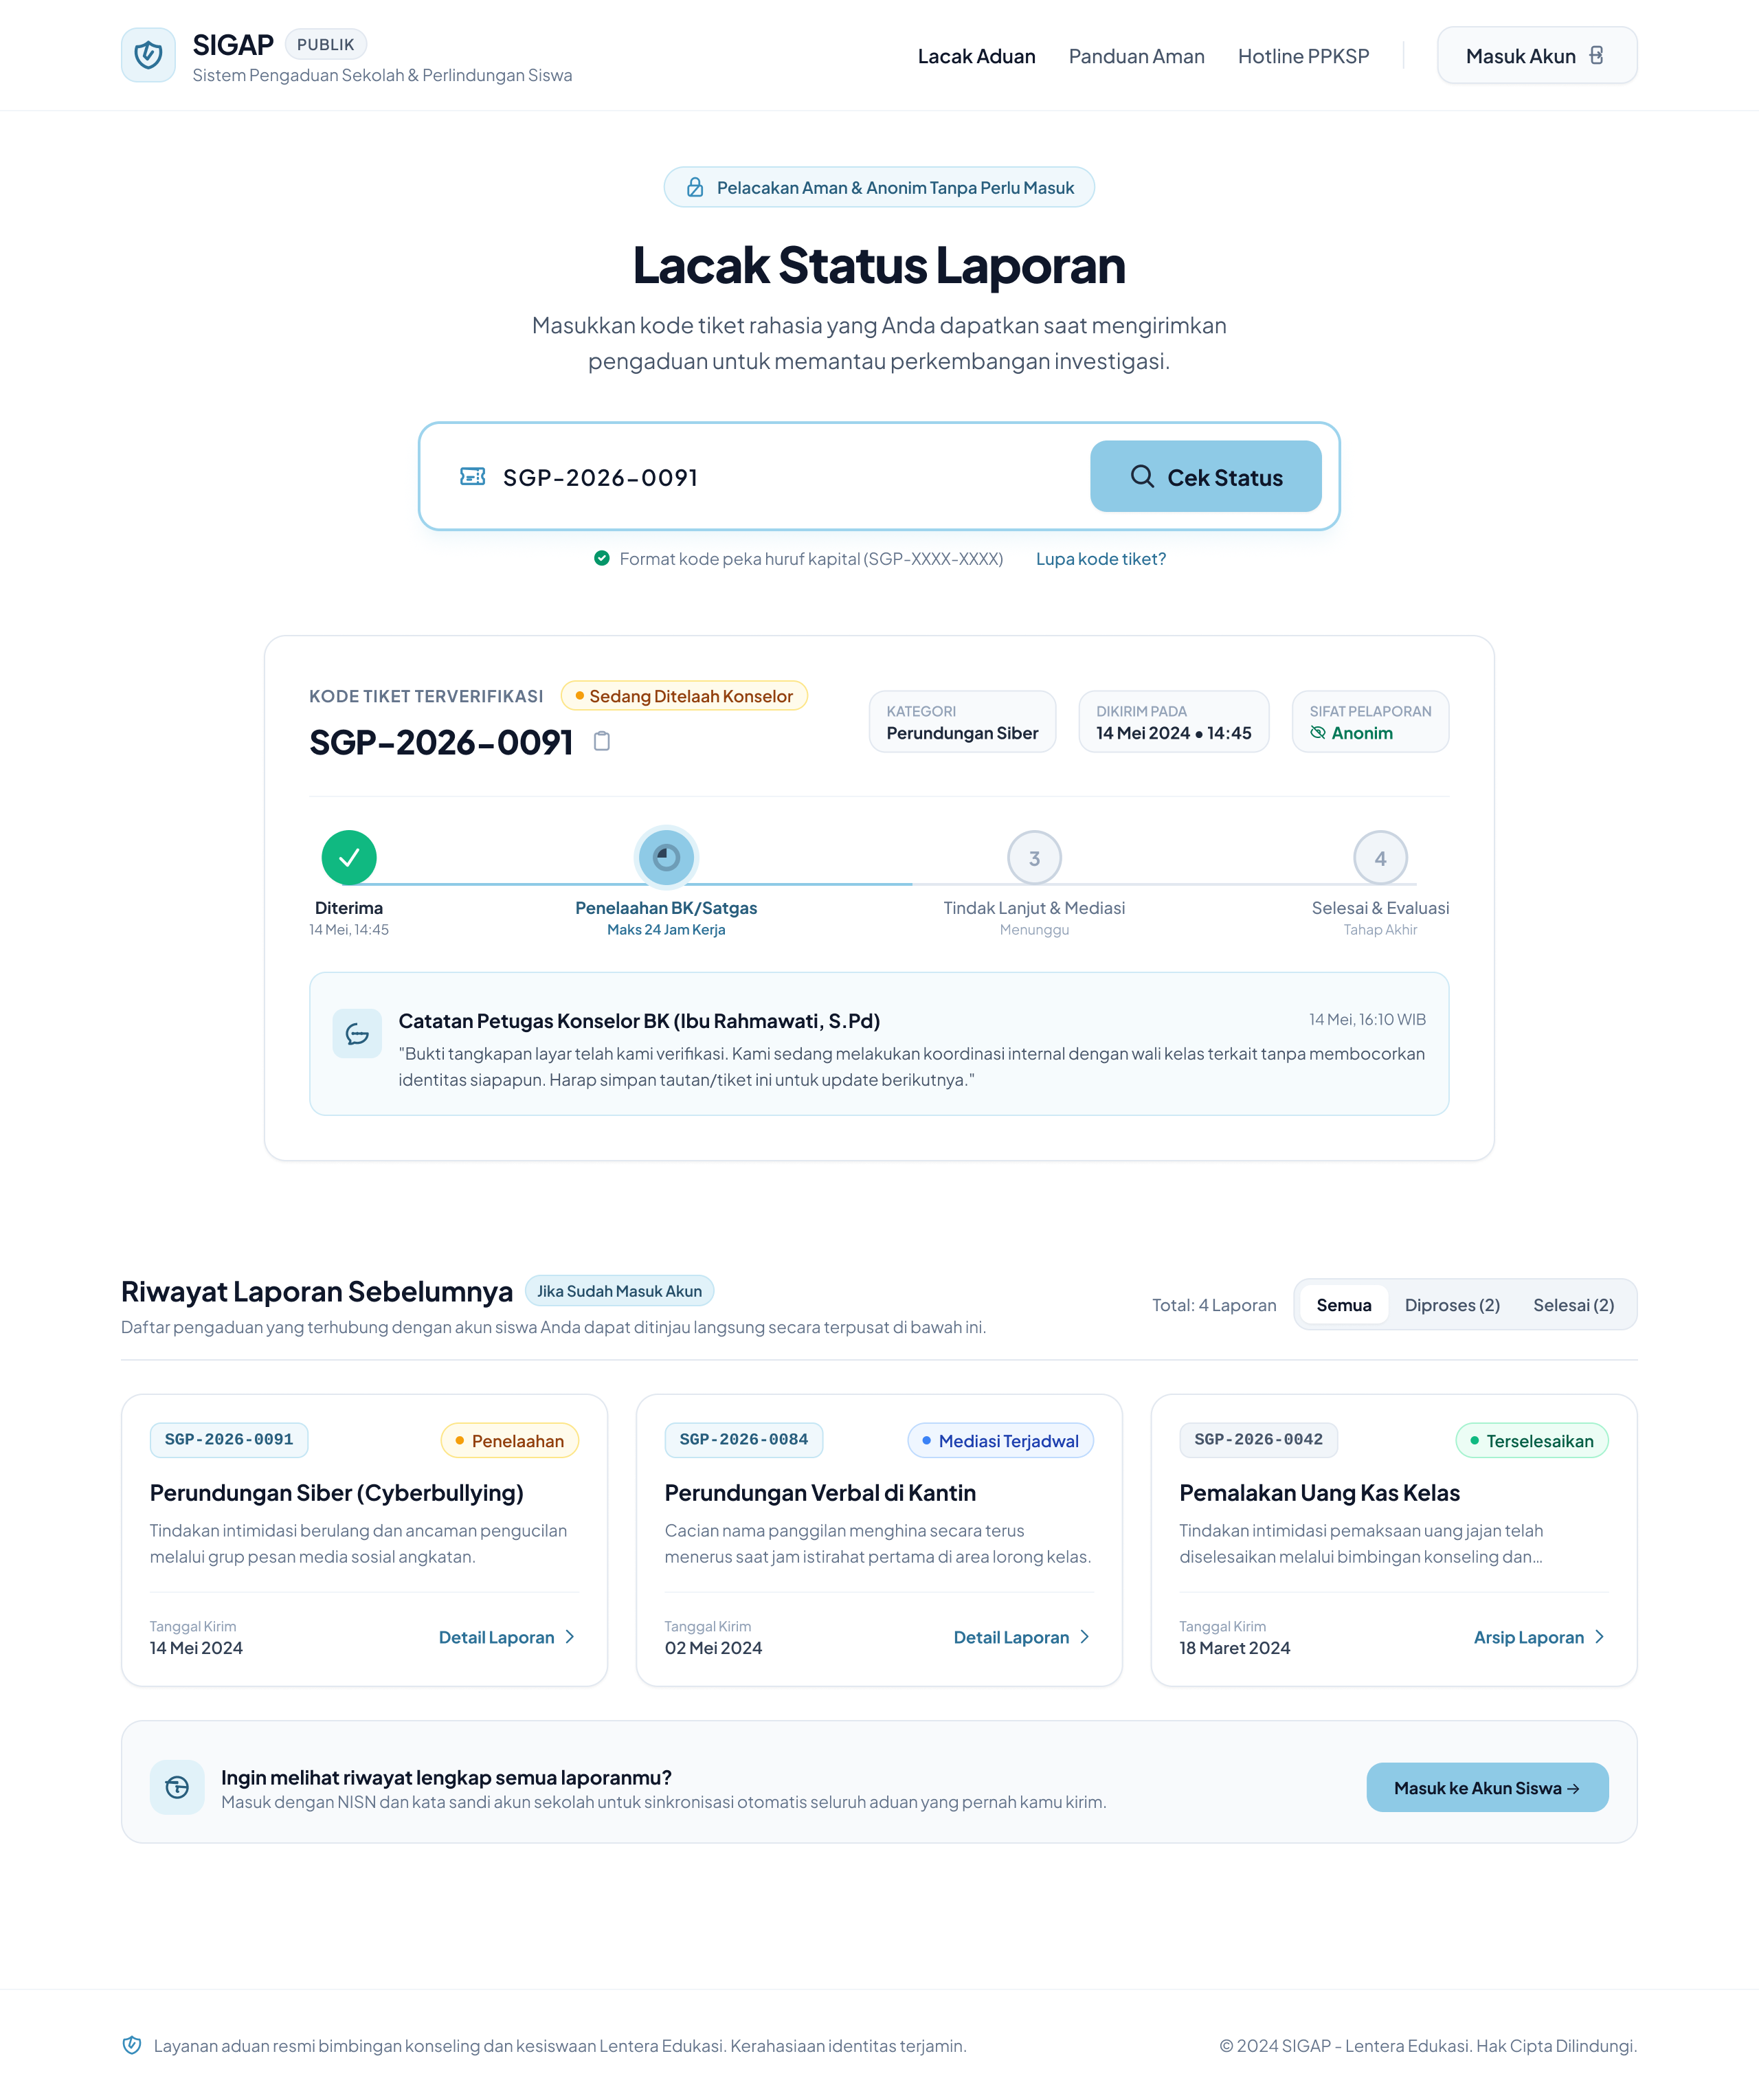
\includegraphics[width=\linewidth,height=0.42\textheight,keepaspectratio]{Frontend/LacakStatusLaporanUser_SIGAP.png}
		\caption{Pelacakan status laporan pengguna siswa}
	\end{figure}
\end{minipage}

\noindent
\begin{minipage}[t]{0.48\linewidth}
	\begin{figure}[H]
		\centering
		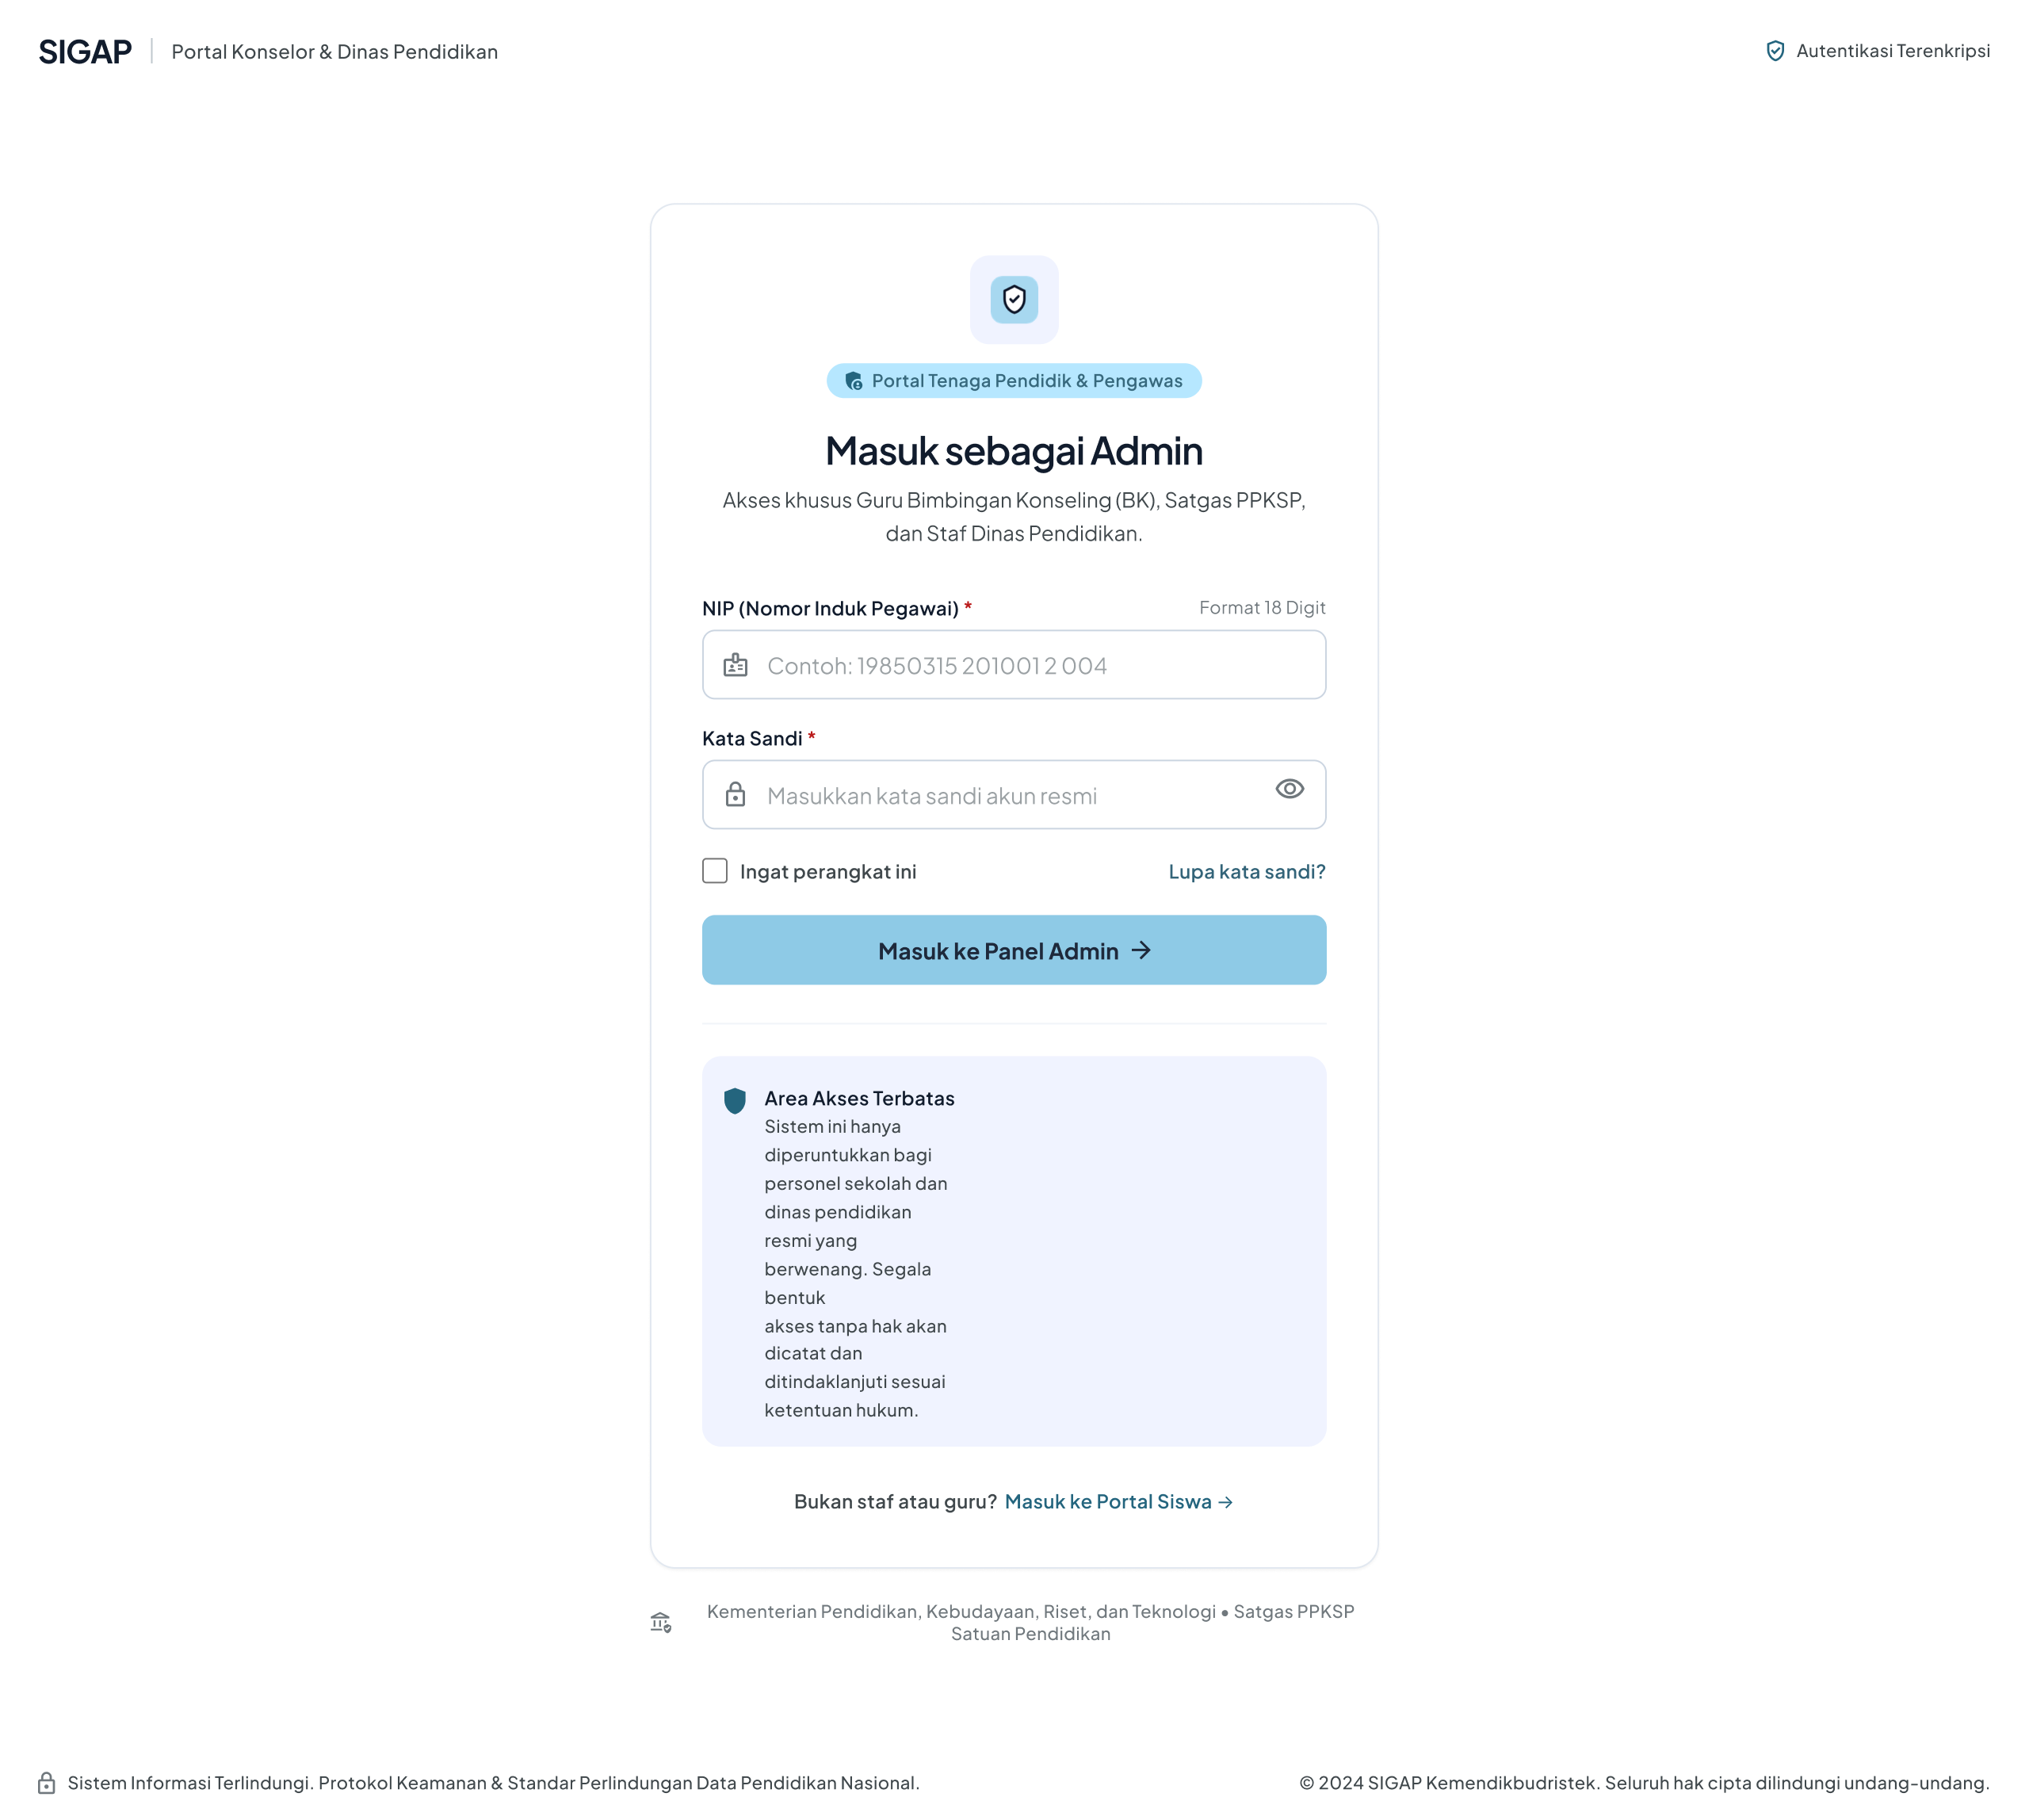
\includegraphics[width=\linewidth,height=0.42\textheight,keepaspectratio]{Frontend/OnBoardingAdmin_SIGAP.png}
		\caption{Onboarding admin}
	\end{figure}
\end{minipage}
\hfill
\begin{minipage}[t]{0.48\linewidth}
	\begin{figure}[H]
		\centering
		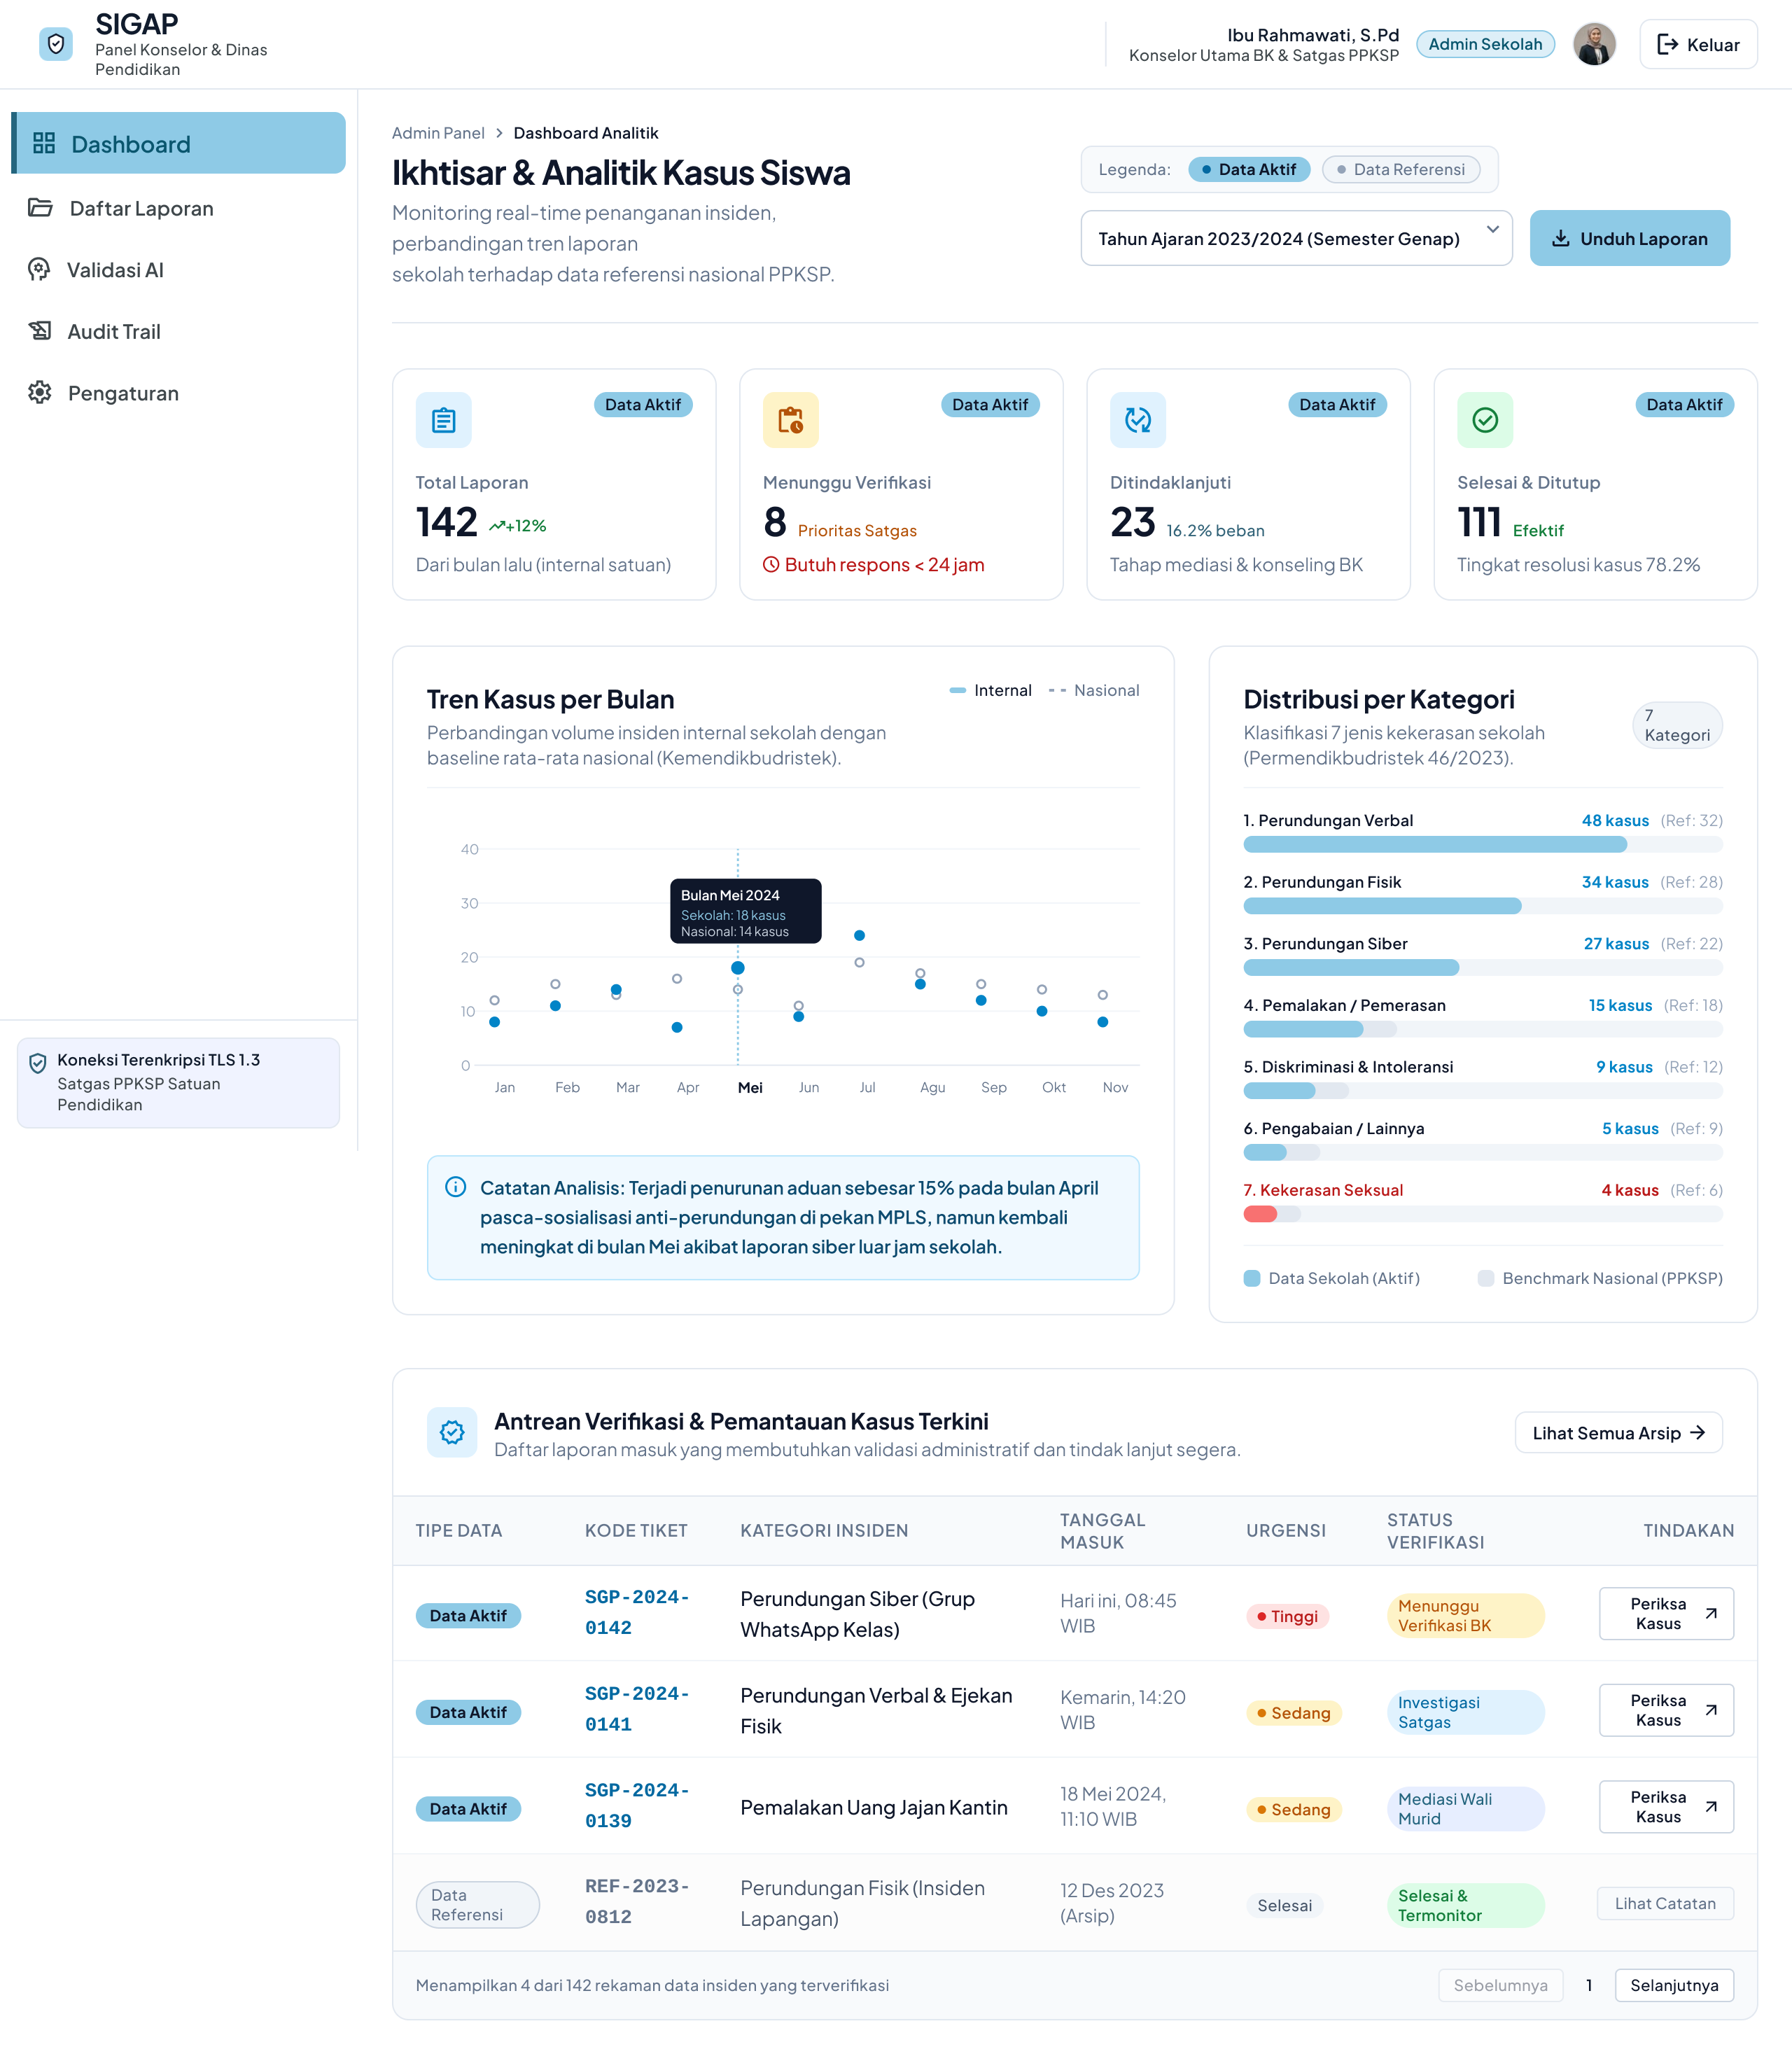
\includegraphics[width=\linewidth,height=0.42\textheight,keepaspectratio]{Frontend/DashboardAdmin_SIGAP.png}
		\caption{Dashboard admin}
	\end{figure}
\end{minipage}

\noindent
\begin{minipage}[t]{0.48\linewidth}
	\begin{figure}[H]
		\centering
		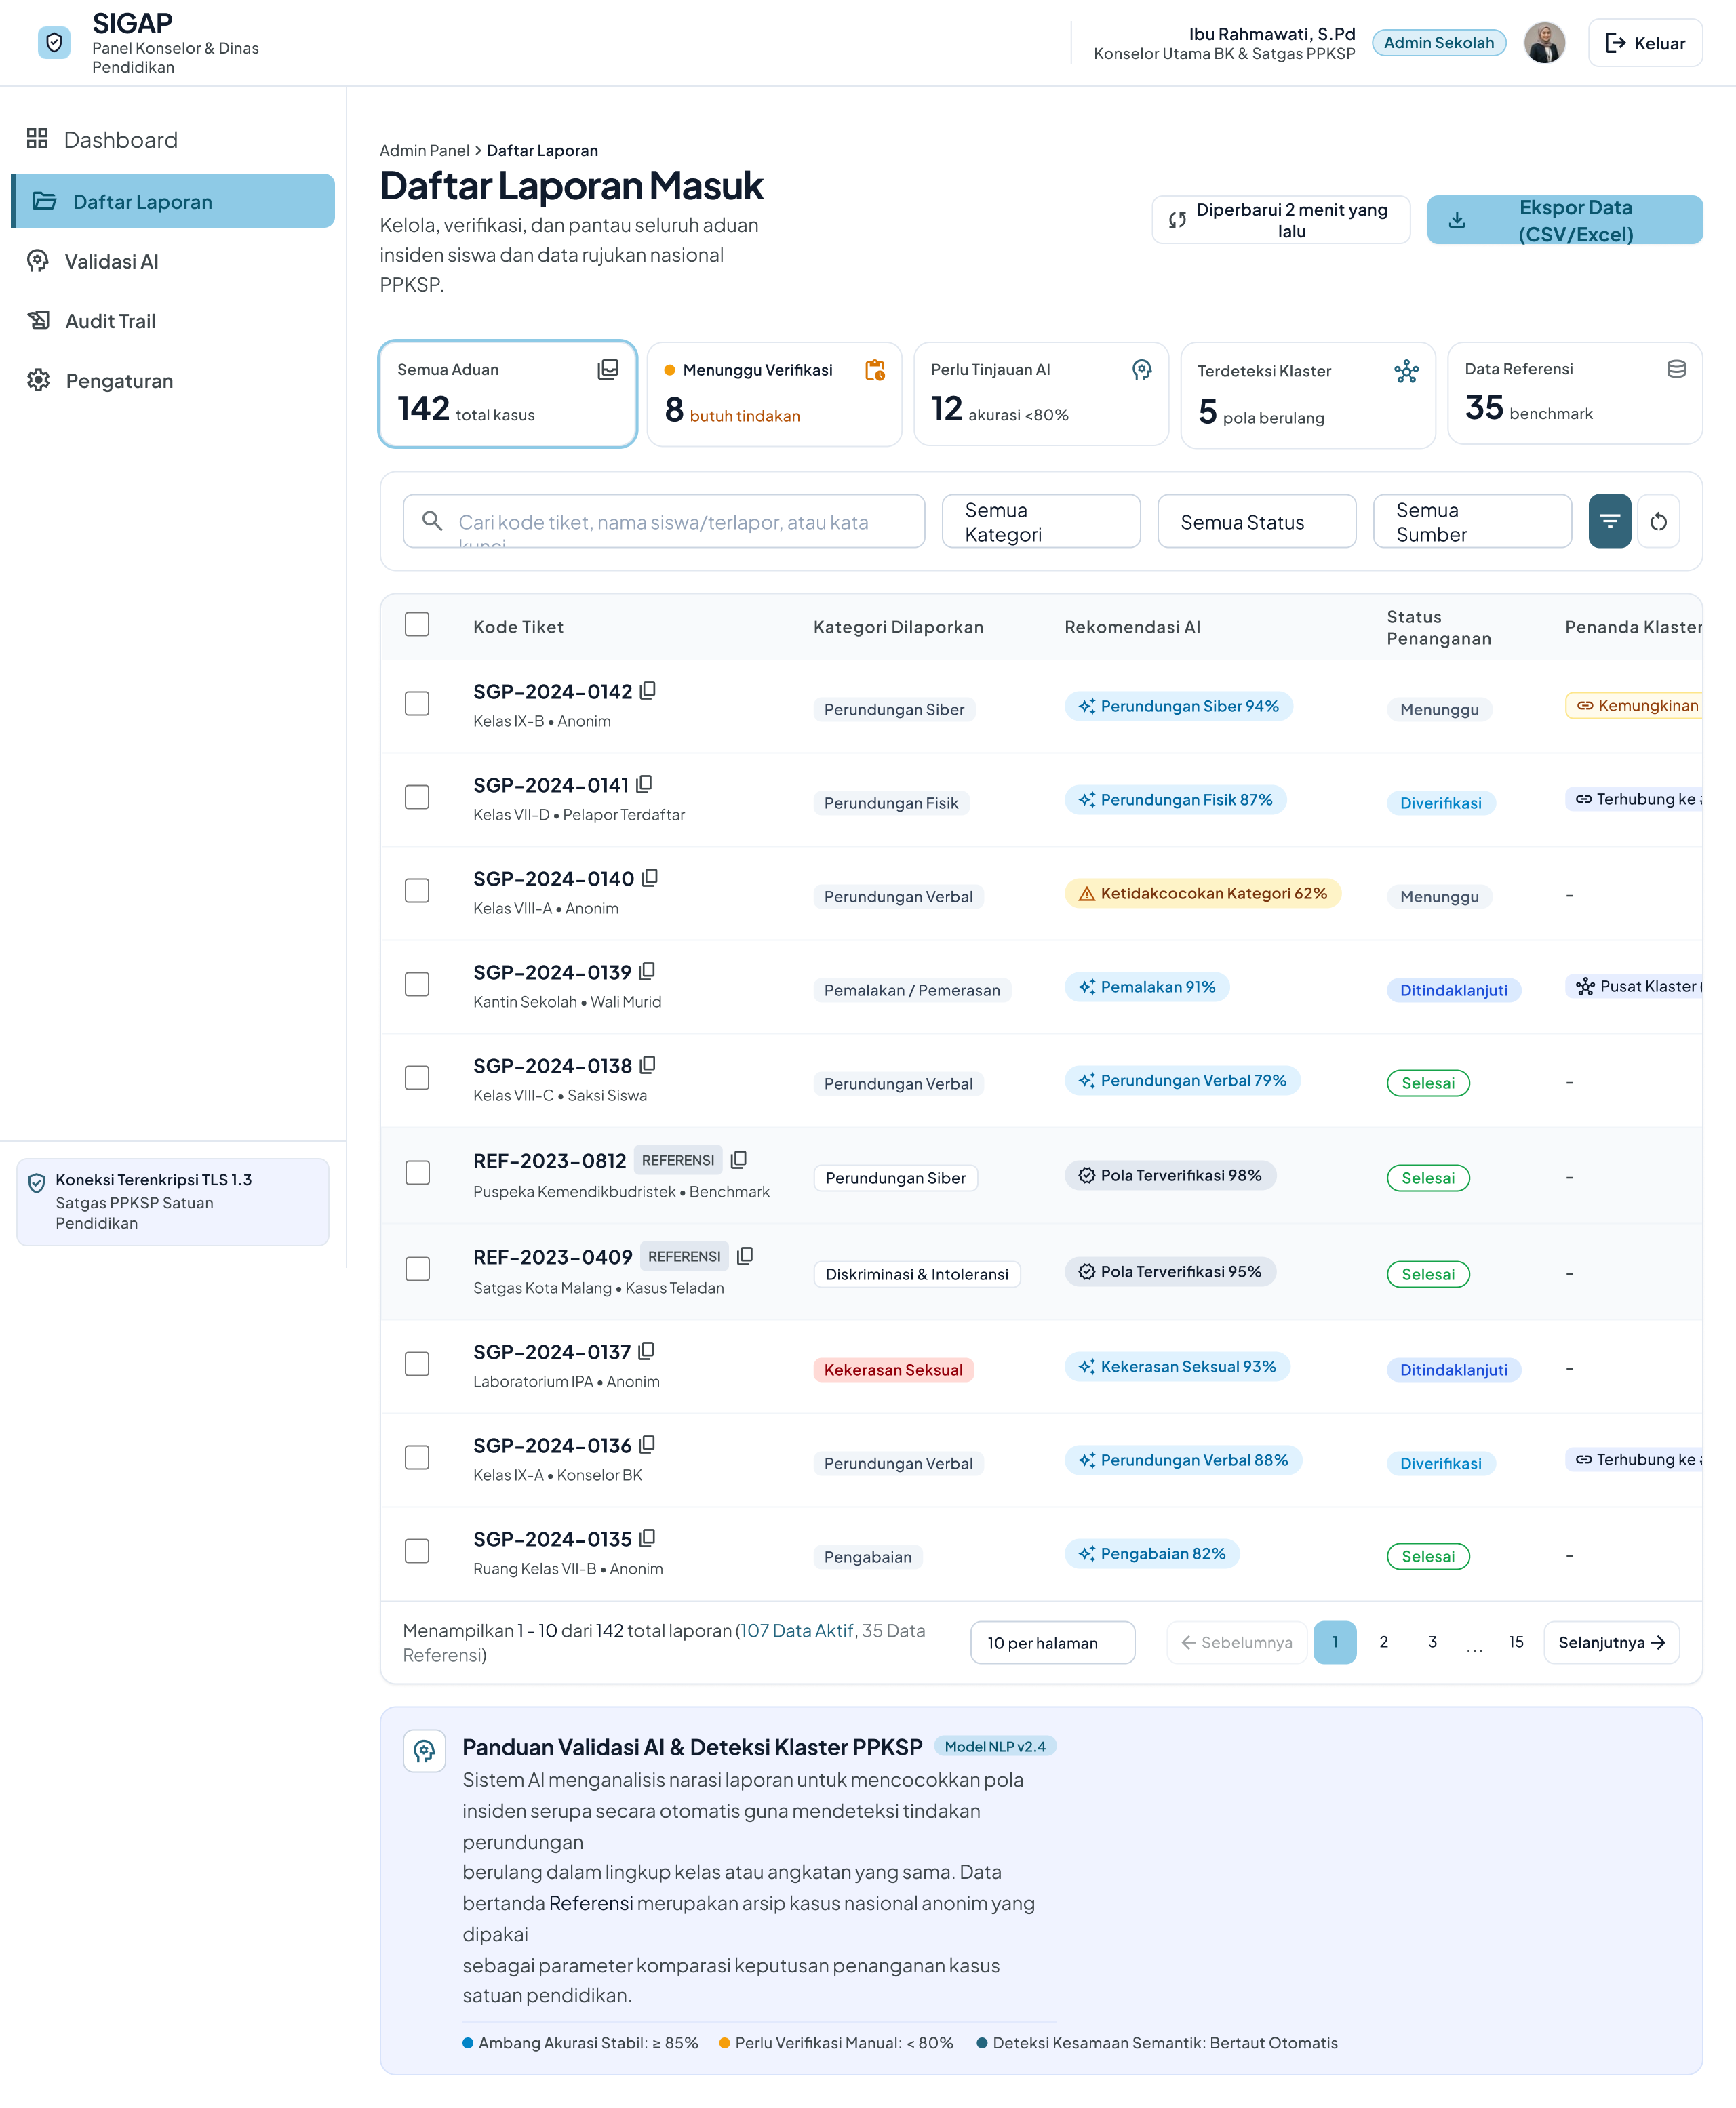
\includegraphics[width=\linewidth,height=0.42\textheight,keepaspectratio]{Frontend/DaftarLaporanMasukAdmin_SIGAP.png}
		\caption{Daftar laporan masuk admin}
	\end{figure}
\end{minipage}
\hfill
\begin{minipage}[t]{0.48\linewidth}
	\begin{figure}[H]
		\centering
		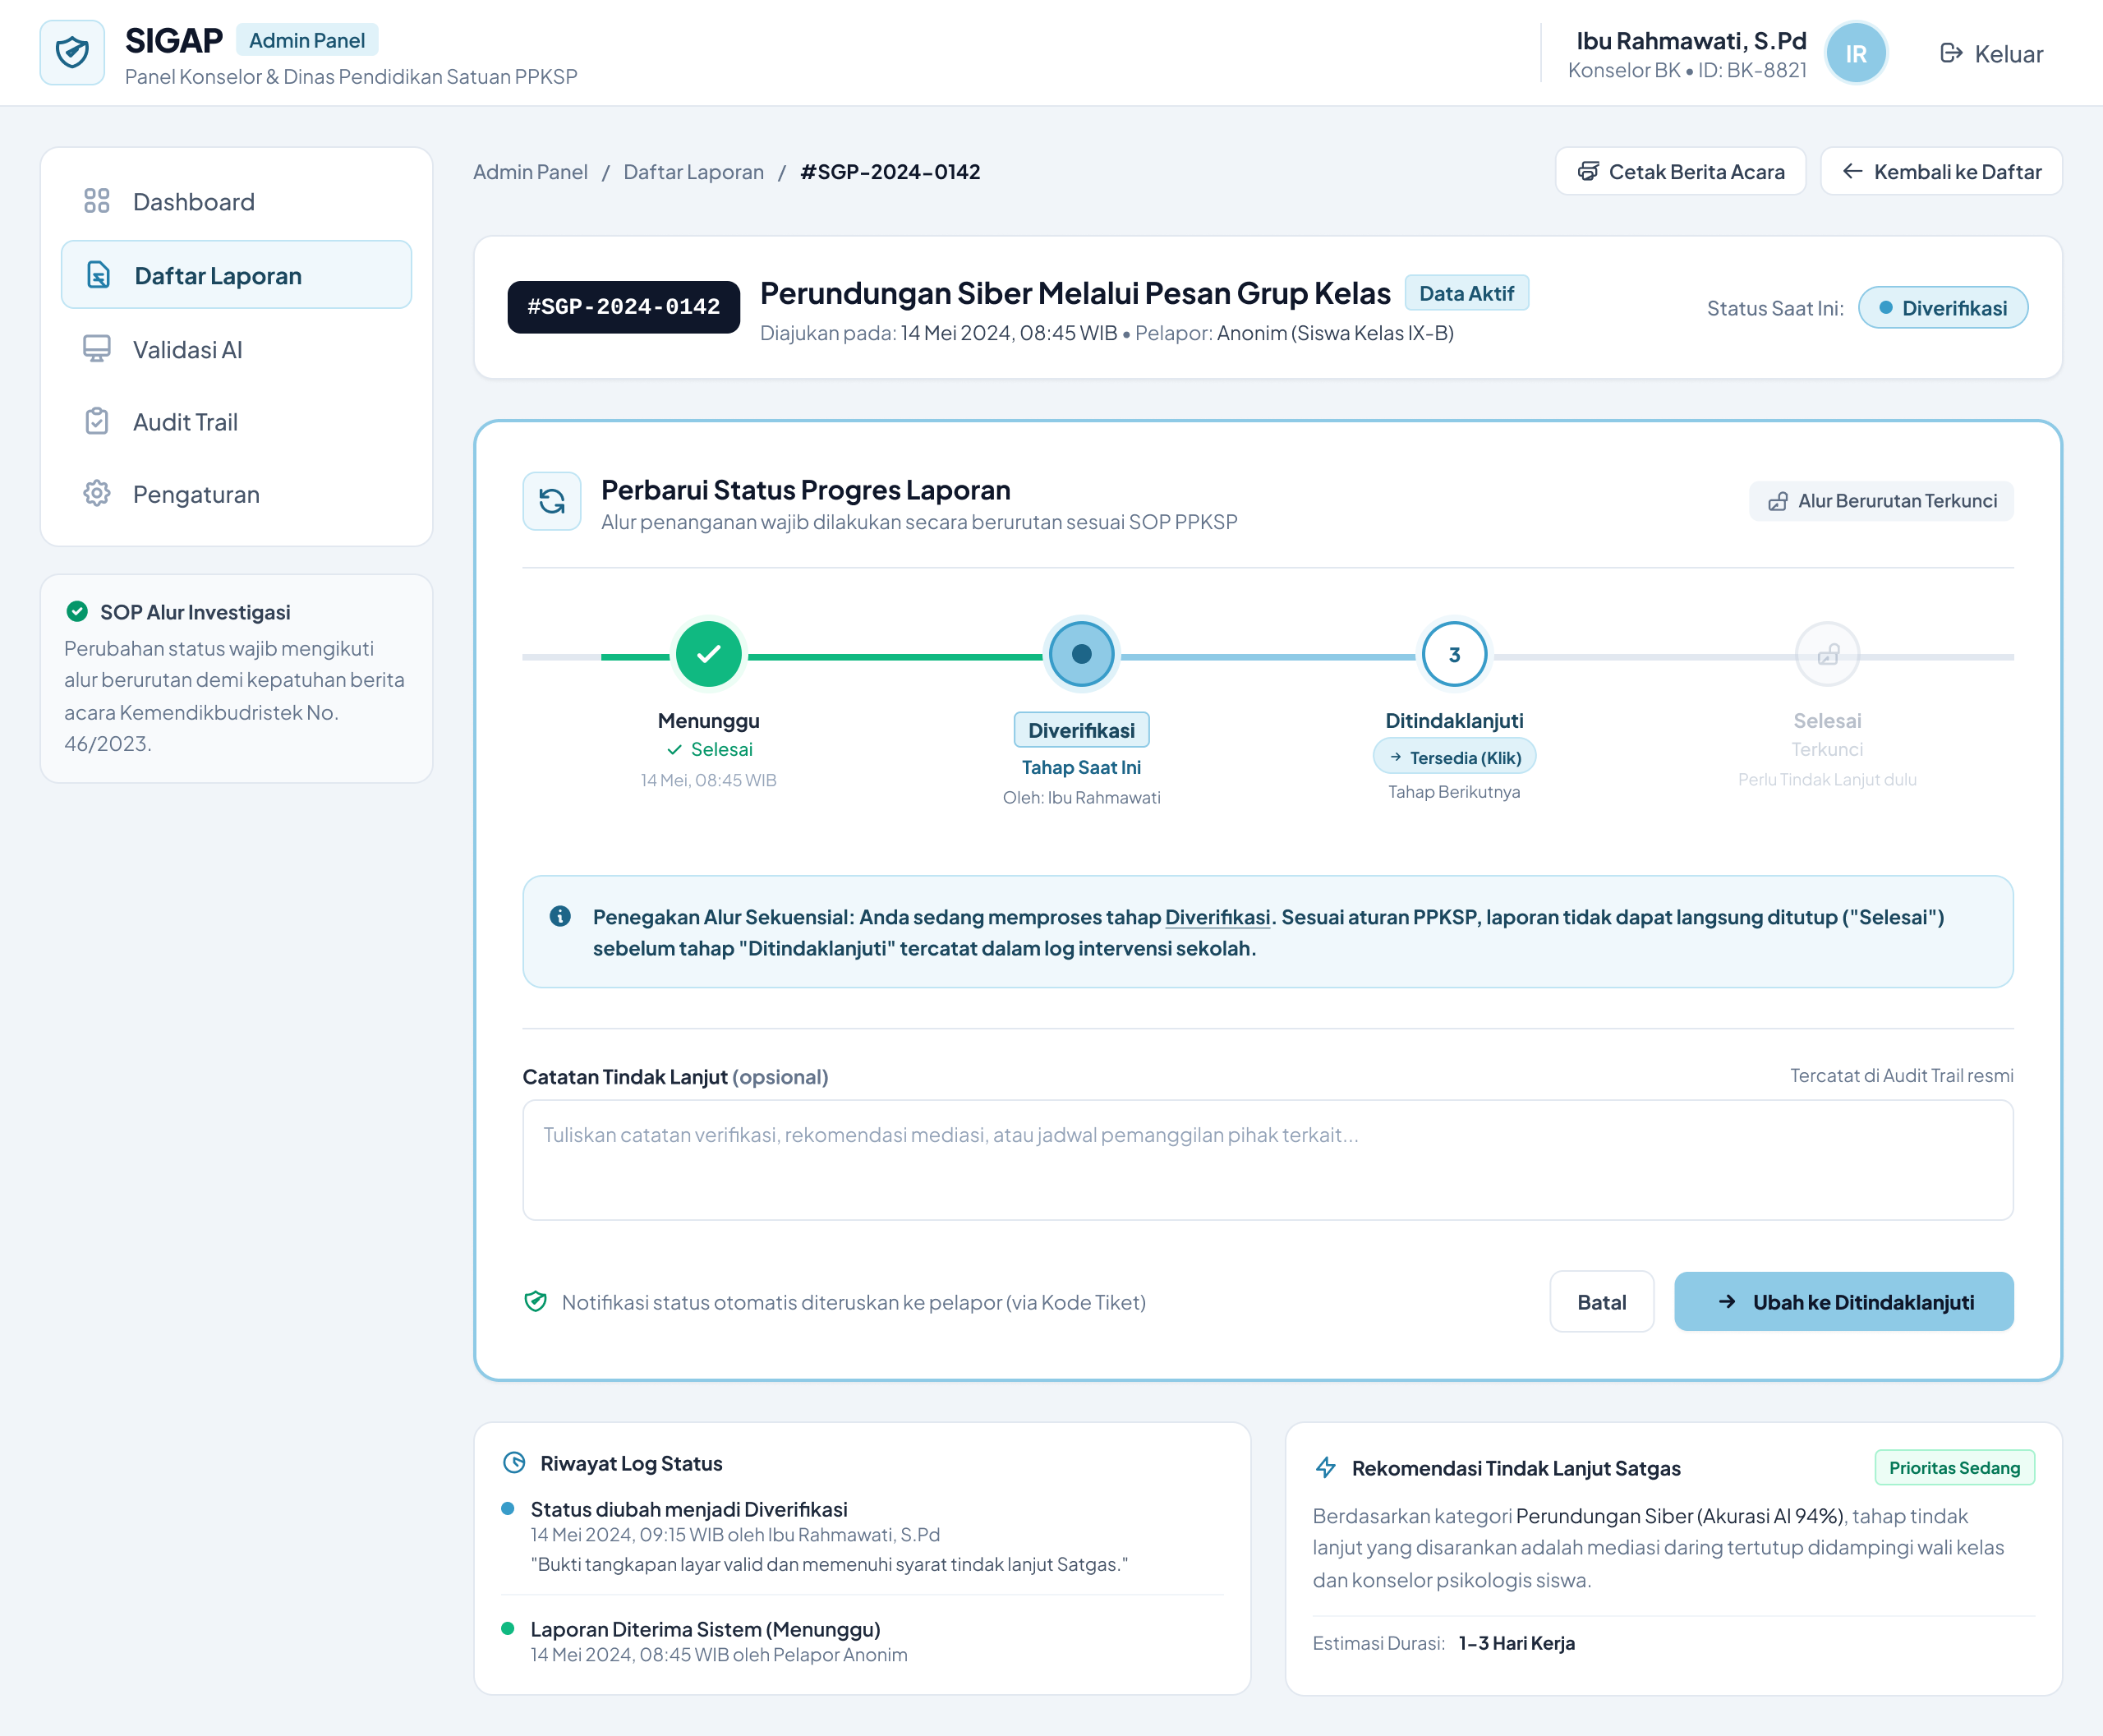
\includegraphics[width=\linewidth,height=0.42\textheight,keepaspectratio]{Frontend/StatusLaporanAdmin_SIGAP.png}
		\caption{Status laporan pada sisi admin}
	\end{figure}
\end{minipage}

\noindent
\begin{minipage}[t]{0.48\linewidth}
	\begin{figure}[H]
		\centering
		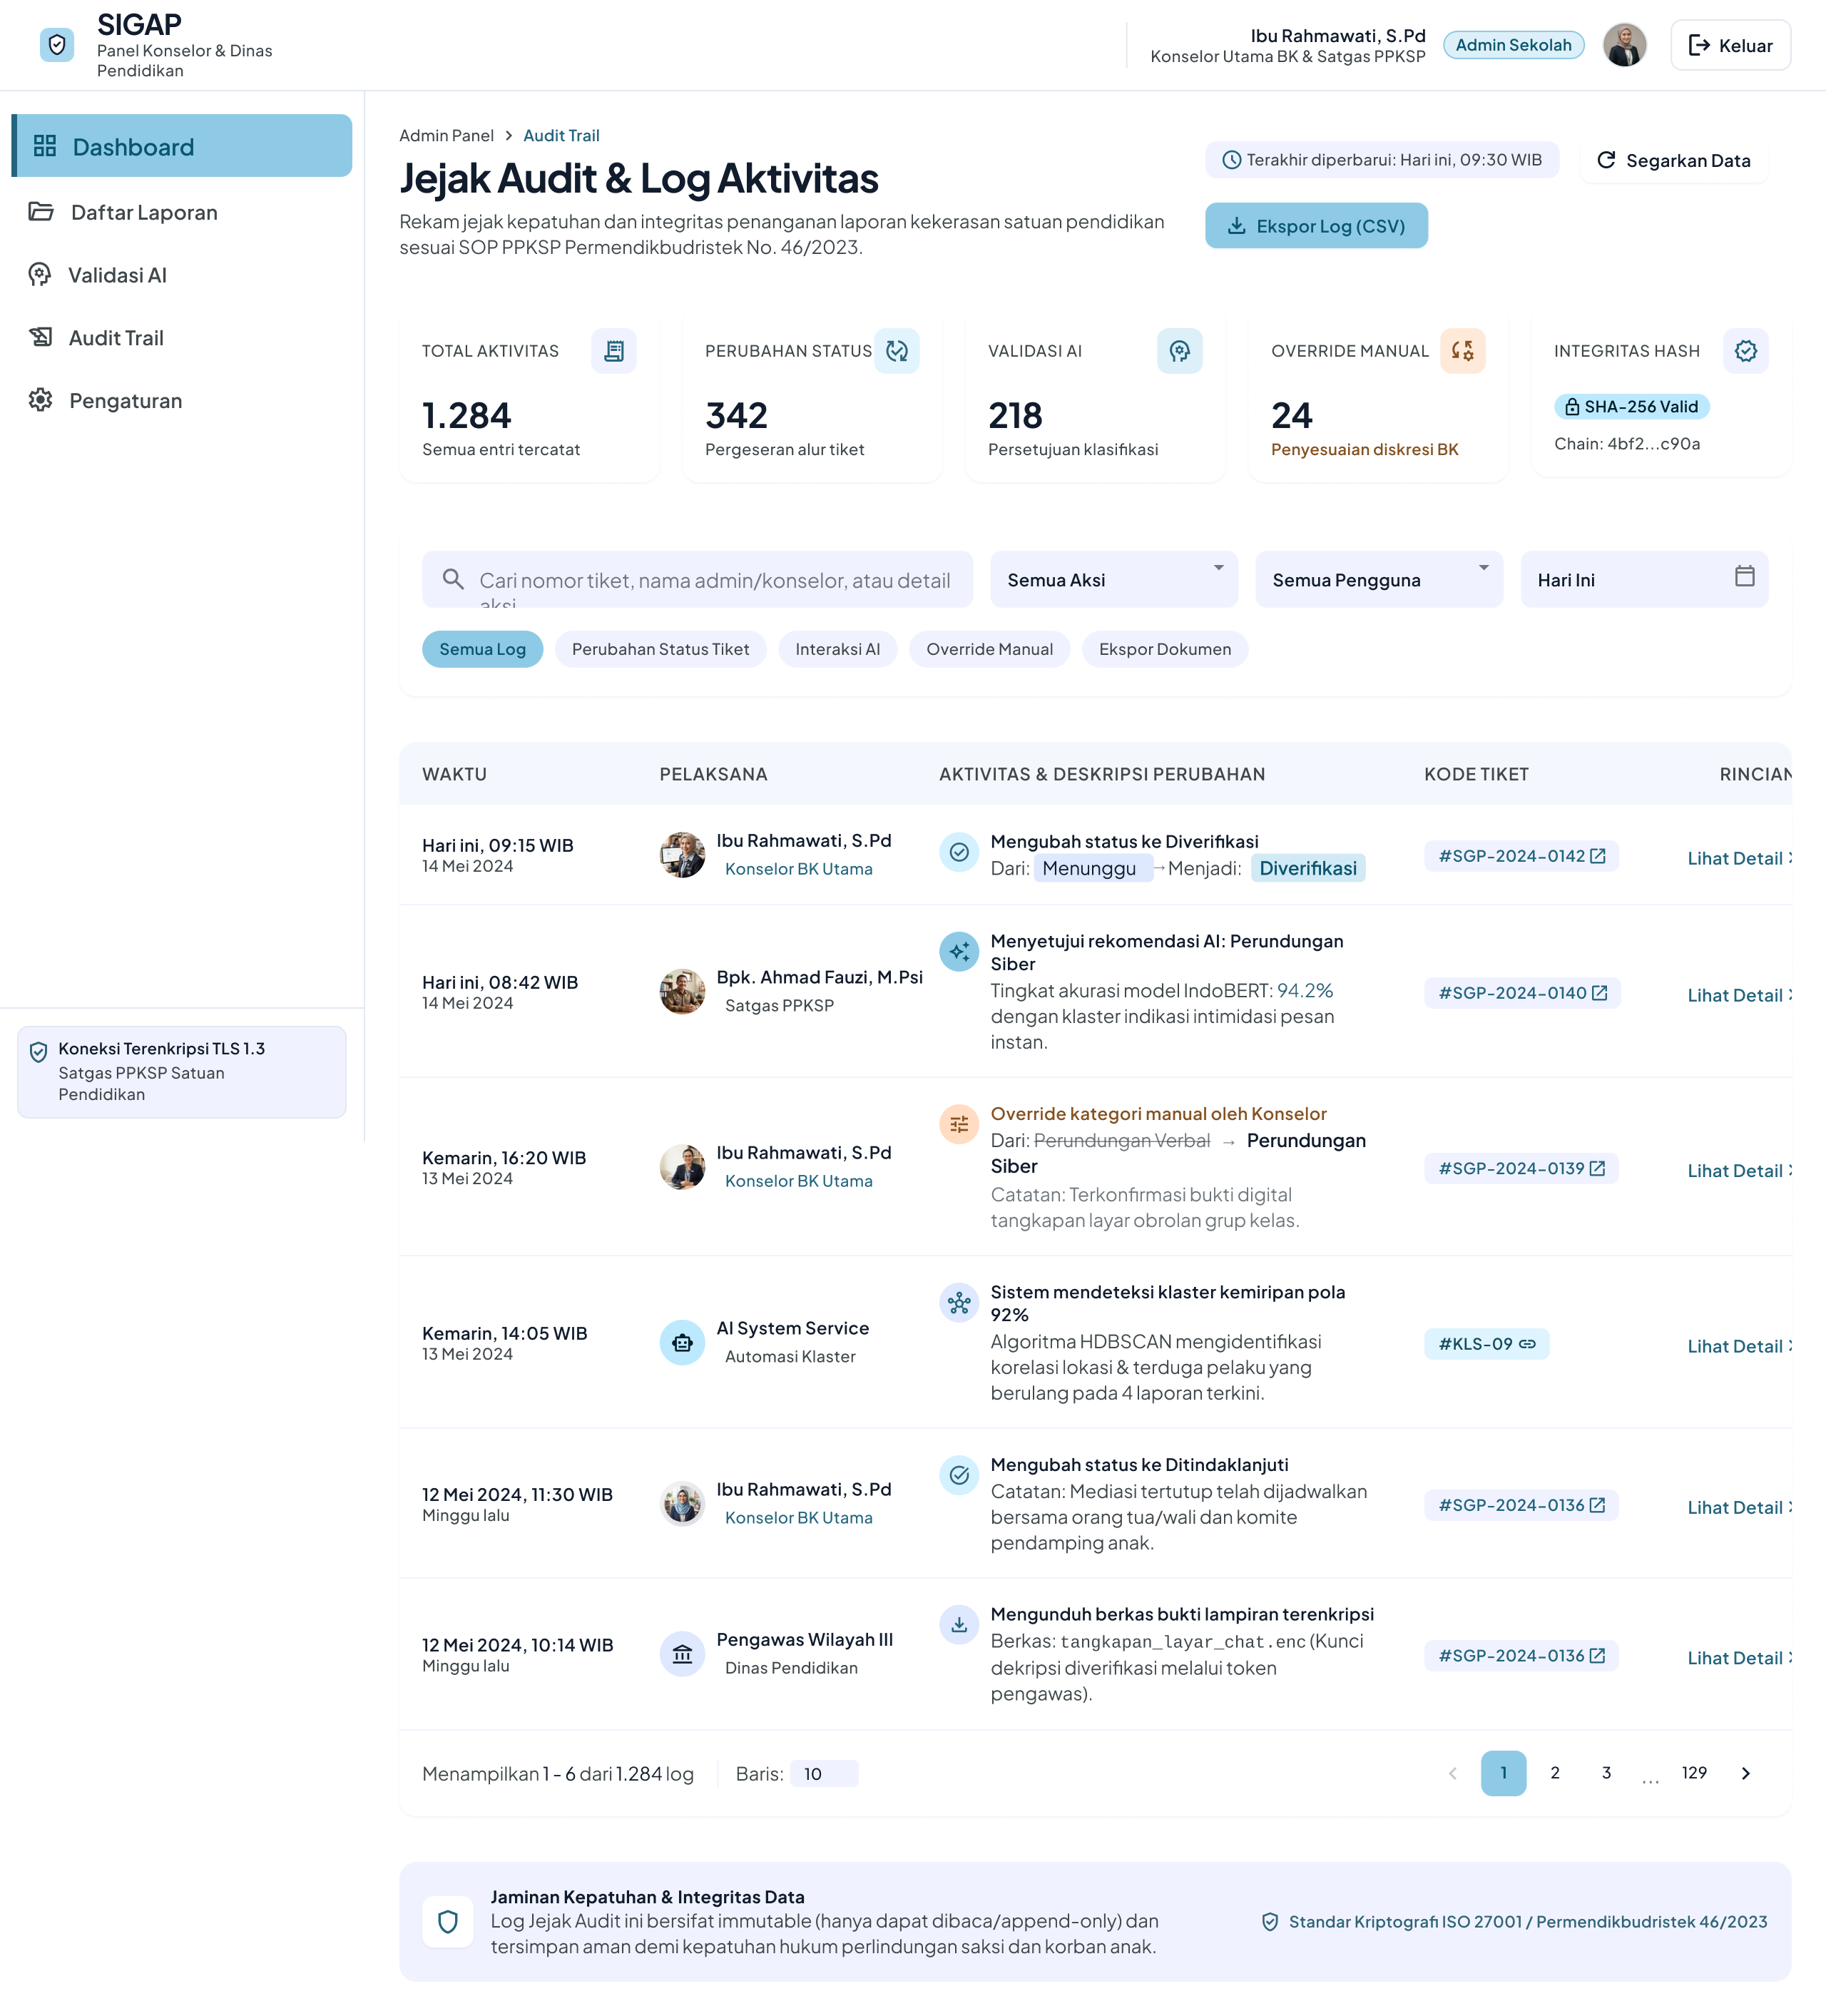
\includegraphics[width=\linewidth,height=0.42\textheight,keepaspectratio]{Frontend/JejakAuditAdmin_SIGAP.png}
		\caption{Jejak audit admin}
	\end{figure}
\end{minipage}

\end{document}